\documentclass[14pt, a4paper]{article}
\usepackage{minitoc}
\usepackage[left=3.00cm, right=2.5cm, top=2.00cm, bottom=2.00cm]{geometry}
\usepackage{amsmath}
\usepackage{amssymb}
\usepackage{amsthm}
\usepackage{mathtools}
\usepackage{graphicx}
%\usepackage{algpseudocode}
%\usepackage{algorithm}
\usepackage[ruled,vlined,linesnumbered]{algorithm2e}
\usepackage{blindtext}
\usepackage{setspace}
\usepackage[utf8]{inputenc}
\usepackage[utf8]{vietnam}
\usepackage[center]{caption}
\usepackage[shortlabels]{enumitem}
\usepackage{fancyhdr} % header, footer
\usepackage{hyperref} % loại bỏ border với mục lục và công thức
\usepackage[nonumberlist, nopostdot, nogroupskip]{glossaries}
\usepackage{glossary-superragged}
\usepackage{tikz,tkz-tab}
\usepackage{pythonhighlight}
\setglossarystyle{superraggedheaderborder}
\pagestyle{fancy}
%\usepackage[style=numeric,sortcites]{biblatex}
%\addbibresource{ref.bib}
%\usepackage[numbers]{natbib}
\usepackage{indentfirst}
\usepackage[natbib,backend=biber,style=ieee, sorting=ynt]{biblatex}

\usepackage{caption}
\usepackage{subcaption}

\bibliography{ref.bib}

\graphicspath{{./figures/}}

\fancyhf{}
%\rhead{\textbf{Môn học: Các phương pháp thống kê hiện đại trong nghiên cứu Xã hội học}}
\lhead{\textbf{GVHD: TS. Trịnh Quốc Anh}}
\rfoot{\thepage}
\lfoot{\textbf{Học viên thực hiện: Nguyễn Chí Thanh - 21007925}}
\renewcommand{\headrulewidth}{0.4pt}
\renewcommand{\footrulewidth}{0.4pt}
%
%\numberwithin{equation}{section}
%\numberwithin{algorithm}{section}
%\numberwithin{figure}{section}
%
%\setlength{\parindent}{0.5cm}
%
%\setcounter{secnumdepth}{3} % Cho phép subsubsection trong report
%\setcounter{tocdepth}{3} % Chèn subsubsection vào bảng mục lục

%\newtheorem{dl}{Định lý}
%\newtheorem{md}{Mệnh đề}
%\newtheorem{bd}{Bổ đề}
%\newtheorem{dn}{Định nghĩa}
%\newtheorem{hq}{Hệ quả}

%\newtheorem{baitap}{Bài tập}
%\newtheorem*{loigiai}{Lời giải}

%\numberwithin{dl}{section}
%\numberwithin{md}{section}
%\numberwithin{bd}{section}
%\numberwithin{dn}{section}
%\numberwithin{hq}{section}

\setlength{\parindent}{0cm}

\newtheorem{dl}{Định lý}
\newtheoremstyle{sltheorem}
{}                % Space above
{}                % Space below
{\normalfont}        % Theorem body font % (default is "\upshape")
{}                % Indent amount
{\bfseries}       % Theorem head font % (default is \mdseries)
{.}               % Punctuation after theorem head % default: no punctuation
{ }               % Space after theorem head
{}                % Theorem head spec
\theoremstyle{sltheorem}
\newtheorem{baitap}{Bài tập}
\newtheoremstyle{soltheorem}
{}                % Space above
{}                % Space below
{\normalfont}        % Theorem body font % (default is "\upshape")
{}                % Indent amount
{\bfseries}       % Theorem head font % (default is \mdseries)
{.}               % Punctuation after theorem head % default: no punctuation
{\newline}               % Space after theorem head
{}                % Theorem head spec
\theoremstyle{soltheorem}
\newtheorem*{loigiai}{Lời giải}

\onehalfspacing

\begin{document}
\begin{titlepage}

    \newcommand{\HRule}{\rule{\linewidth}{0.5mm}} % Defines a new command for the horizontal lines, change thickness here

    \center % Center everything on the page

    %----------------------------------------------------------------------------------------
    %	HEADING SECTIONS
    %----------------------------------------------------------------------------------------
    \textsc{\LARGE Đại học Quốc Gia Hà Nội}\\[0.5cm]
    \textsc{\LARGE Trường đại học Khoa học tự nhiên}\\[0.5cm] % Name of your university/college
    \textsc{\LARGE Khoa Toán - Cơ - Tin học}\\[0.5cm]

    
\includegraphics[scale=0.2]{HUS-logo.jpg}\\[0.5cm]

    \textsc{\Large Chuyên ngành: Khoa học dữ liệu}\\[0.5cm] % Major heading such as course name


    %----------------------------------------------------------------------------------------
    %	TITLE SECTION
    %----------------------------------------------------------------------------------------

    \HRule \\[0.4cm]
    { \huge \bfseries Bài tập môn học}\\[0.4cm] % Title of your document
    \HRule \\[1.5cm]

    \textsc{\Large Môn học: Các phương pháp thống kê hiện đại \\ trong nghiên cứu Xã hội học}\\[1cm] % Minor heading such as course title


    \textsc{\Large Bài tập số 3}\\[1cm]


    %----------------------------------------------------------------------------------------
    %	AUTHOR SECTION
    %----------------------------------------------------------------------------------------
    \begin{minipage}{0.4\textwidth}
        \begin{flushleft} \large
        \emph{Giảng viên hướng dẫn:} \\
        TS. Trịnh Quốc Anh % Supervisor's Name
        \end{flushleft}
    \end{minipage}\\[0.5cm]

    \begin{minipage}{0.4\textwidth}
    \begin{flushleft} \large
    \emph{Học viên thực hiện:}\\
    Nguyễn Chí Thanh \\
    MSHV: 21007925 \\ % Your name
    Lớp: Khoa học dữ liệu - K4
    \end{flushleft}
    \end{minipage}


    % If you don't want a supervisor, uncomment the two lines below and remove the section above
    %\Large \emph{Author:}\\
    %John \textsc{Smith}\\[3cm] % Your name

    %----------------------------------------------------------------------------------------
    %	DATE SECTION
    %----------------------------------------------------------------------------------------

    % I don't want day because it is English
    % {\large \today}\\[2cm] % Date, change the \today to a set date if you want to be precise

    %----------------------------------------------------------------------------------------
    %	LOGO SECTION
    %----------------------------------------------------------------------------------------

    %\includegraphics{logo/rsz_3logo-khtn.png}\\[1cm] % Include a department/university logo - this will require the graphicx package

    %----------------------------------------------------------------------------------------

    \vfill % Fill the rest of the page with whitespace

\end{titlepage}

\nocite{*}

\newpage

\begin{baitap}
    Áp dụng các phương pháp Ridge, LASSO, và PCA cho dữ liệu Sonar.

    Hãy so sánh các kết quả thu được và biện luận để đưa ra mô hình phù hợp nhất.
\end{baitap}

\begin{loigiai}
    Hàm mất mát của mô hình logistic regression:
    \begin{equation*}
        \mathcal{L} = -\dfrac{1}{N}\sum_{i=1}^N (y_i \log \hat{y}_i + (1-y_i)\log(1-\hat{y}_i)) 
    \end{equation*}

    với $\hat{y}=p(y=1\vert \bold{x})=f(\bold{x}) = \sigma(w_0 + w_1 x_1 + w_2 x_2 + \dots w_n x_n) = \sigma(\bold{w}^T \bold{x})$ là kết quả đầu ra của mô hình logistic tương ứng với đầu vào $\bold{x}$.

    Hàm mất mát của phương pháp Ridge:

    \begin{equation*}
        \mathcal{L}_{\mathrm{Ridge}} = -\dfrac{1}{N}\sum_{i=1}^N (y_i \log \hat{y}_i + (1-y_i)\log(1-\hat{y}_i)) + \lambda \lVert \bold{w} \rVert_2^2
    \end{equation*}

    Hàm mất mát của phương pháp LASSO:

    \begin{equation*}
        \mathcal{L}_{\mathrm{Ridge}} = -\dfrac{1}{N}\sum_{i=1}^N (y_i \log \hat{y}_i + (1-y_i)\log(1-\hat{y}_i)) + \lambda \lVert \bold{w} \rVert_1
    \end{equation*}

    Để xây dựng mô hình, ta sẽ sử dụng các hướng sau:

        \begin{itemize}
            \item Mô hình bao gồm tất cả các biến (đặc trưng) từ tập dữ liệu.
            \item Mô hình bao gồm các đặc trưng được trích xuất từ thuật toán PCA giữa lại 95 \% thông tin.
            \item Mô hình gồm các biến được chọn từ hàm step() để lựa chọn mô hình trong ngôn ngữ R.
        \end{itemize}

    Dữ liệu trước khi đưa vào hàm step() trong R được tiền xử lý theo hai cách:

    \begin{itemize}
        \item Min max scaling (minmax)
        \item Standardize
    \end{itemize}

    Ta kiểm định các hệ số của mô hình forward sử dụng likelihood ratio test:

\begin{verbatim}
    anova(minmax_m.f, test="Chisq")
\end{verbatim}

    \begin{verbatim}
Df	Deviance	Resid. Df	Resid. Dev	Pr(>Chi)
<int>	<dbl>	<int>	<dbl>	<dbl>
NULL	NA	NA	207	287.40621	NA
V11	1	45.813415	206	241.59279	1.300698e-11
V47	1	19.278348	205	222.31444	1.129803e-05
V36	1	14.276700	204	208.03774	1.578062e-04
V45	1	11.188262	203	196.84948	8.231642e-04
V4	1	7.877562	202	188.97192	5.005192e-03
V15	1	7.147110	201	181.82481	7.508488e-03
V21	1	10.009874	200	171.81494	1.557032e-03
V51	1	5.049499	199	166.76544	2.463306e-02
V8	1	6.307759	198	160.45768	1.202107e-02
V49	1	4.305721	197	156.15196	3.798439e-02
V50	1	3.675029	196	152.47693	5.523328e-02
V1	1	4.399958	195	148.07697	3.593981e-02
V3	1	3.994465	194	144.08250	4.564995e-02
V52	1	4.131899	193	139.95061	4.208211e-02
V54	1	5.142063	192	134.80854	2.335288e-02
V23	1	5.266855	191	129.54169	2.173524e-02
V29	1	3.784617	190	125.75707	5.172573e-02
V31	1	5.069299	189	120.68777	2.435323e-02
V12	1	5.208250	188	115.47952	2.247995e-02
V30	1	3.796447	187	111.68307	5.136148e-02
V32	1	6.695459	186	104.98762	9.665880e-03
V53	1	3.503780	185	101.48384	6.122894e-02
V7	1	3.585955	184	97.89788	5.826991e-02
V16	1	4.186234	183	93.71165	4.075352e-02
V9	1	3.377209	182	90.33444	6.610391e-02
V26	1	3.287893	181	87.04654	6.979253e-02
V37	1	3.799709	180	83.24684	5.126148e-02
V34	1	2.558428	179	80.68841	1.097077e-01
V35	1	3.043974	178	77.64443	8.103731e-02
V38	1	2.682565	177	74.96187	1.014522e-01
V6	1	2.916942	176	72.04493	8.765385e-02
V40	1	2.279184	175	69.76574	1.311208e-01
V59	1	2.302910	174	67.46283	1.291319e-01
V19	1	2.118068	173	65.34476	1.455701e-01
V56	1	2.415767	172	62.92900	1.201192e-01
    \end{verbatim}

    \begin{verbatim}
anova(standardize_m.f, test="Chisq")
    \end{verbatim}

    \begin{verbatim}
Df	Deviance	Resid. Df	Resid. Dev	Pr(>Chi)
<int>	<dbl>	<int>	<dbl>	<dbl>
NULL	NA	NA	207	287.40621	NA
V11	1	45.813415	206	241.59279	1.300698e-11
V47	1	19.278348	205	222.31444	1.129803e-05
V36	1	14.276700	204	208.03774	1.578062e-04
V45	1	11.188262	203	196.84948	8.231642e-04
V4	1	7.877562	202	188.97192	5.005192e-03
V15	1	7.147110	201	181.82481	7.508488e-03
V21	1	10.009874	200	171.81494	1.557032e-03
V51	1	5.049499	199	166.76544	2.463306e-02
V8	1	6.307759	198	160.45768	1.202107e-02
V49	1	4.305721	197	156.15196	3.798439e-02
V50	1	3.675029	196	152.47693	5.523328e-02
V1	1	4.399958	195	148.07697	3.593981e-02
V3	1	3.994465	194	144.08250	4.564995e-02
V52	1	4.131899	193	139.95061	4.208211e-02
V54	1	5.142063	192	134.80854	2.335288e-02
V23	1	5.266855	191	129.54169	2.173524e-02
V29	1	3.784617	190	125.75707	5.172573e-02
V31	1	5.069299	189	120.68777	2.435323e-02
V12	1	5.208250	188	115.47952	2.247995e-02
V30	1	3.796447	187	111.68307	5.136148e-02
V32	1	6.695459	186	104.98762	9.665880e-03
V53	1	3.503780	185	101.48384	6.122894e-02
V7	1	3.585955	184	97.89788	5.826991e-02
V16	1	4.186234	183	93.71165	4.075352e-02
V9	1	3.377209	182	90.33444	6.610391e-02
V26	1	3.287893	181	87.04654	6.979253e-02
V37	1	3.799709	180	83.24684	5.126148e-02
V34	1	2.558428	179	80.68841	1.097077e-01
V35	1	3.043974	178	77.64443	8.103731e-02
V38	1	2.682565	177	74.96187	1.014522e-01
V6	1	2.916942	176	72.04493	8.765385e-02
V40	1	2.279184	175	69.76574	1.311208e-01
V59	1	2.302910	174	67.46283	1.291319e-01
V19	1	2.118068	173	65.34476	1.455701e-01
V56	1	2.415767	172	62.92900	1.201192e-01
    \end{verbatim}

    Ta nhận thấy đa số các biến đều đóng góp vai trò đáng kể trong mô hình trừ một số biến như biến V38, V40, V59, V19, V56.
    Bảng phương sai của mô hình minmax\_mf và standardize\_mf gần như giống hệt nhau.

    \begin{figure}[h!]
        \centering
        \begin{subfigure}[b]{0.4\textwidth}
            \centering
            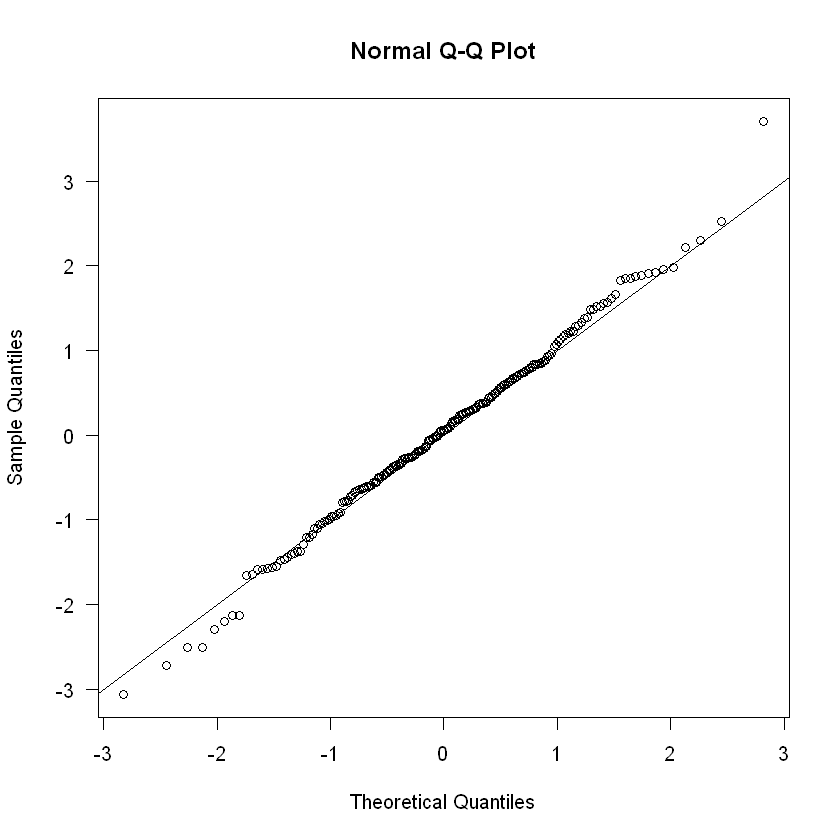
\includegraphics[width=\textwidth]{figures/minmax_mf_quantile_resid.png}
            \caption{Quantile residual của mô hình forward (dữ liệu được tiền xử lý minmax)}
        \end{subfigure}
        \hfill
        \begin{subfigure}[b]{0.4\textwidth}
            \centering
            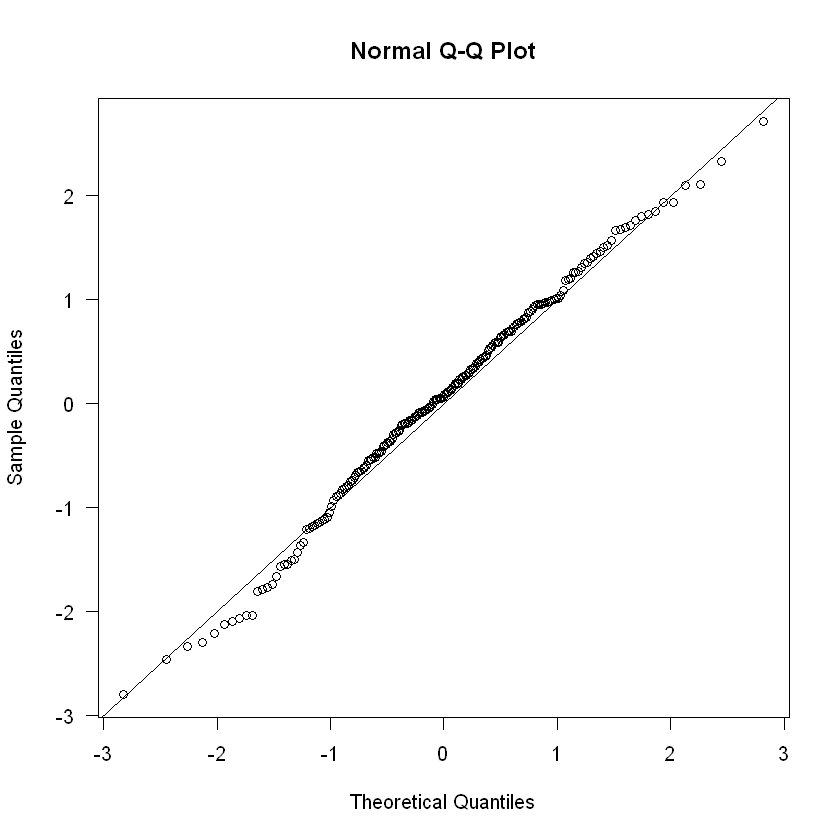
\includegraphics[width=\textwidth]{figures/standardize_mf_quantile_resid.png}
            \caption{Quantile residual của mô hình forward (dữ liệu được tiền xử lý standardize)}
        \end{subfigure}
        \caption{Quantile residual của mô hình forward}
        \label{fig:Quantile-resid-mf}
    \end{figure}

    Hình \ref{fig:Quantile-resid-mf} cho ta thấy đồ thị Q-Q plot của mô hình forward.
    Các điểm quantile residual đa số nằm sát trên đường thẳng chuẩn nhưng có đuôi khá dài.

    \begin{figure}[h!]
        \centering
        \begin{subfigure}[b]{0.4\textwidth}
            \centering
            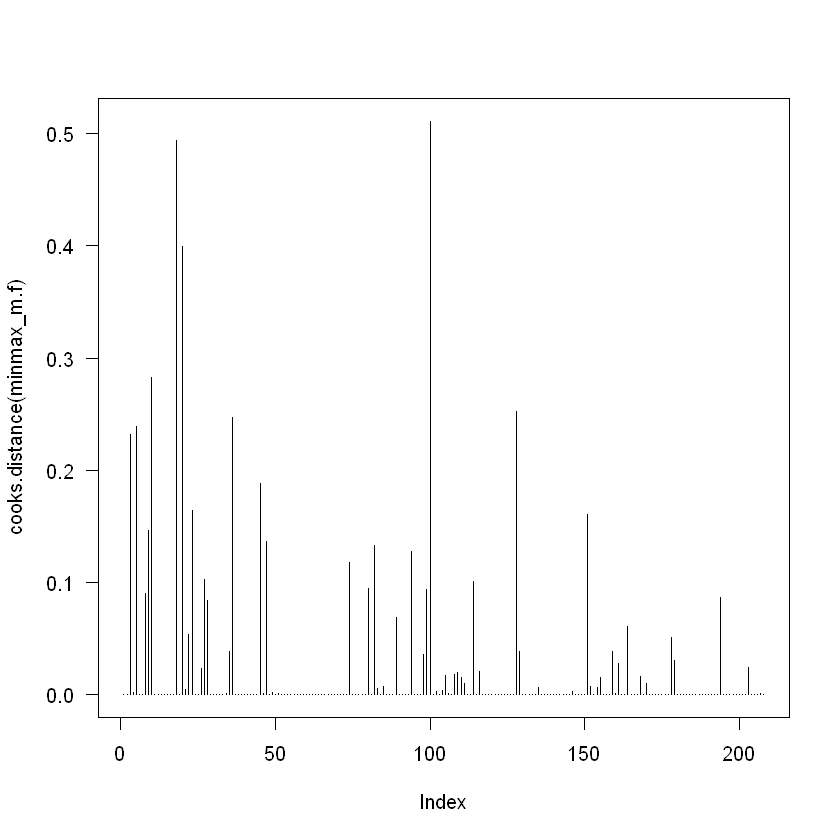
\includegraphics[width=\textwidth]{figures/minmax_mf_cooks.png}
            \caption{Cooks distance của mô hình forward (dữ liệu được tiền xử lý minmax)}
        \end{subfigure}
        \hfill
        \begin{subfigure}[b]{0.4\textwidth}
            \centering
            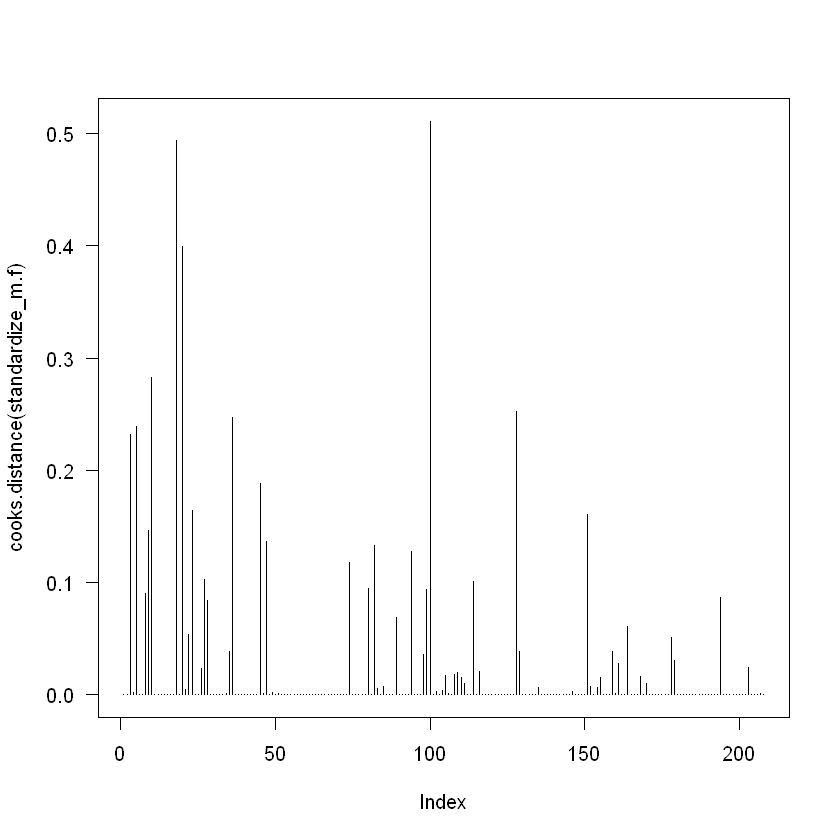
\includegraphics[width=\textwidth]{figures/standardize_mf_cooks.png}
            \caption{Cooks distance của mô hình forward (dữ liệu được tiền xử lý standardize)}
        \end{subfigure}
        \caption{Cooks distance của mô hình forward}
        \label{fig:Cooks-distance-mf}
    \end{figure}

    Hình \ref{fig:Cooks-distance-mf} cho ta biểu diễn Cooks distance của các ví dụ học trong tập dữ liệu.
    Để một ví dụ học được xem là một điểm ngoại lai thì Cook distance của phần tử phải lớn hơn n phân vị mức 0.5 của phân phối Fisher(p, n-p).
    Ta tính phân vị mức của các mô hình trên rơi vào khoảng 0.98.
    Như vậy mô hình forward không có điểm ngoại lai nào.


    \begin{figure}[h!]
        \centering
        \begin{subfigure}[b]{0.4\textwidth}
            \centering
            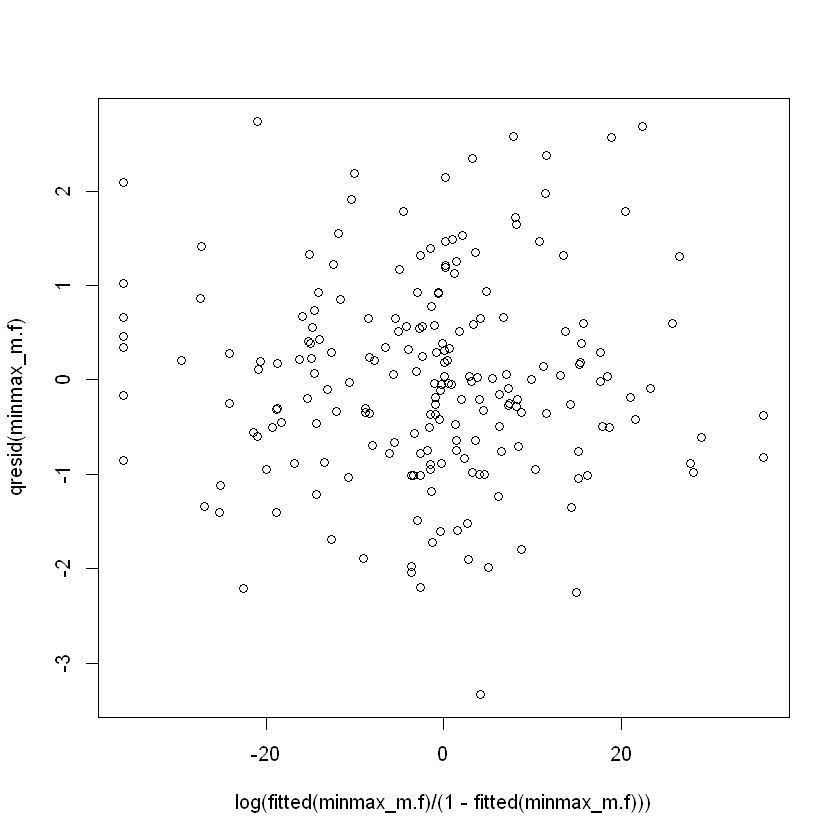
\includegraphics[width=\textwidth]{figures/minmax_mf_fitted.png}
            \caption{Quantile residual theo fitted value của mô hình forward (dữ liệu được tiền xử lý minmax)}
        \end{subfigure}
        \hfill
        \begin{subfigure}[b]{0.4\textwidth}
            \centering
            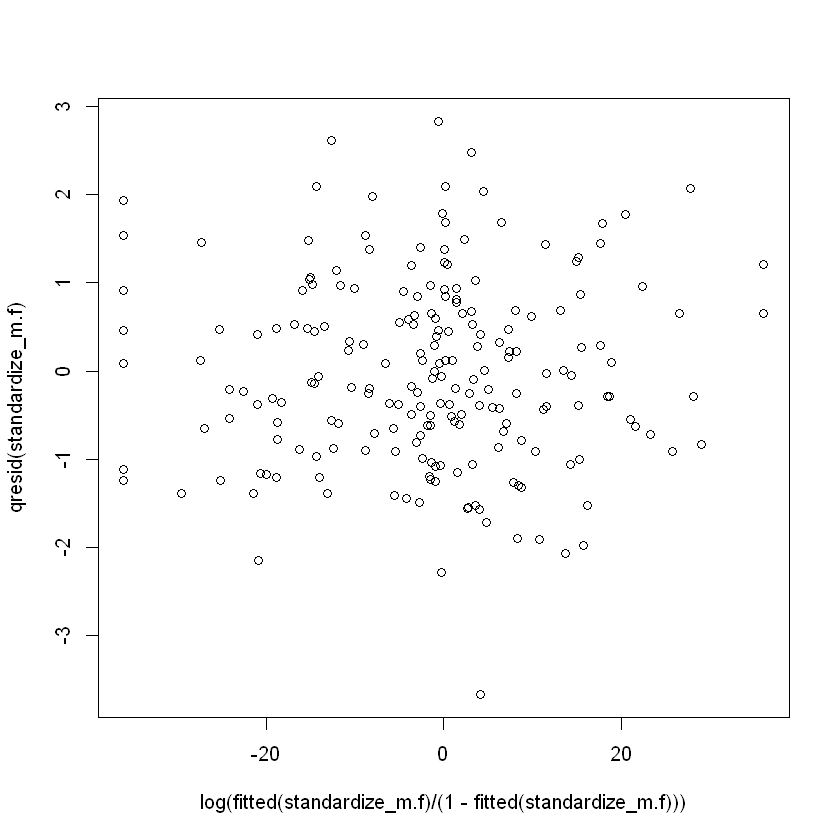
\includegraphics[width=\textwidth]{figures/standardize_mf_fitted.png}
            \caption{Quantile residual theo fitted value của mô hình forward (dữ liệu được tiền xử lý standardize)}
        \end{subfigure}
        \caption{Quantile residual theo fitted value của mô hình forward}
        \label{fig:Quantile-fitted-mf}
    \end{figure}

    Từ hình \ref{fig:Quantile-fitted-mf} ta thấy mô hình forward thể hiện khá tốt các giả định lý
    thuyết khi mà quantile residual ngẫu nhiên xung quanh điểm 0 và so với giá trị $\eta$ (log-odd) của mô
    hình cho thấy các ví dụ độc lập với nhau.

    Ta kiểm định các hệ số của mô hình backward sử dụng likelihood ratio test:

    \begin{verbatim}
anova(minmax_m.b, test="Chisq")
    \end{verbatim}

    \begin{verbatim}
Df	Deviance	Resid. Df	Resid. Dev	Pr(>Chi)
<int>	<dbl>	<int>	<dbl>	<dbl>
NULL	NA	NA	207	2.874062e+02	NA
V1	1	17.713882964	206	2.696923e+02	2.567460e-05
V3	1	0.605538874	205	2.690868e+02	4.364725e-01
V7	1	0.401073639	204	2.686857e+02	5.265353e-01
V9	1	16.415841846	203	2.522699e+02	5.085840e-05
V12	1	18.464018055	202	2.338059e+02	1.731425e-05
V13	1	0.040230414	201	2.337656e+02	8.410307e-01
V14	1	1.482925834	200	2.322827e+02	2.233173e-01
V16	1	2.775377941	199	2.295073e+02	9.572406e-02
V17	1	0.040139972	198	2.294672e+02	8.412072e-01
V18	1	2.554980373	197	2.269122e+02	1.099472e-01
V19	1	9.888496760	196	2.170237e+02	1.663152e-03
V20	1	0.100063203	195	2.169236e+02	7.517538e-01
V21	1	8.718785951	194	2.082049e+02	3.149477e-03
V22	1	4.578958193	193	2.036259e+02	3.236689e-02
V23	1	0.688625865	192	2.029373e+02	4.066322e-01
V24	1	0.007890769	191	2.029294e+02	9.292170e-01
V25	1	0.173935050	190	2.027554e+02	6.766380e-01
V27	1	1.067674920	189	2.016878e+02	3.014712e-01
V29	1	1.307537307	188	2.003802e+02	2.528410e-01
V30	1	0.037764676	187	2.003425e+02	8.459164e-01
V31	1	7.187290937	186	1.931552e+02	7.342175e-03
V32	1	4.891994149	185	1.882632e+02	2.698150e-02
V33	1	6.664572192	184	1.815986e+02	9.834826e-03
V34	1	2.380619623	183	1.792180e+02	1.228488e-01
V37	1	5.647405508	182	1.735706e+02	1.748122e-02
V39	1	3.342750615	181	1.702278e+02	6.750168e-02
V40	1	0.003614541	180	1.702242e+02	9.520592e-01
V41	1	8.616473888	179	1.616077e+02	3.331361e-03
V42	1	4.215551288	178	1.573922e+02	4.005505e-02
V43	1	2.942413740	177	1.544498e+02	8.628171e-02
V46	1	12.732911806	176	1.417169e+02	3.592767e-04
V48	1	18.532618731	175	1.231842e+02	1.670213e-05
V50	1	11.198645365	174	1.119856e+02	8.185707e-04
V51	1	13.815457905	173	9.817014e+01	2.016702e-04
V52	1	24.175881404	172	7.399426e+01	8.792654e-07
V57	1	0.196456219	171	7.379781e+01	6.575966e-01
V58	1	73.797803271	170	2.848136e-06	8.654286e-18
    \end{verbatim}

    \begin{verbatim}
anova(standardize_m.b, test="Chisq")
    \end{verbatim}

    \begin{verbatim}
Df	Deviance	Resid. Df	Resid. Dev	Pr(>Chi)
<int>	<dbl>	<int>	<dbl>	<dbl>
NULL	NA	NA	207	2.874062e+02	NA
V1	1	17.713882964	206	2.696923e+02	2.567460e-05
V3	1	0.605538874	205	2.690868e+02	4.364725e-01
V7	1	0.401073639	204	2.686857e+02	5.265353e-01
V9	1	16.415841846	203	2.522699e+02	5.085840e-05
V12	1	18.464018055	202	2.338059e+02	1.731425e-05
V13	1	0.040230414	201	2.337656e+02	8.410307e-01
V14	1	1.482925834	200	2.322827e+02	2.233173e-01
V16	1	2.775377941	199	2.295073e+02	9.572406e-02
V17	1	0.040139972	198	2.294672e+02	8.412072e-01
V18	1	2.554980373	197	2.269122e+02	1.099472e-01
V19	1	9.888496760	196	2.170237e+02	1.663152e-03
V20	1	0.100063203	195	2.169236e+02	7.517538e-01
V21	1	8.718785951	194	2.082049e+02	3.149477e-03
V22	1	4.578958193	193	2.036259e+02	3.236689e-02
V23	1	0.688625865	192	2.029373e+02	4.066322e-01
V24	1	0.007890769	191	2.029294e+02	9.292170e-01
V25	1	0.173935050	190	2.027554e+02	6.766380e-01
V27	1	1.067674920	189	2.016878e+02	3.014712e-01
V29	1	1.307537307	188	2.003802e+02	2.528410e-01
V30	1	0.037764676	187	2.003425e+02	8.459164e-01
V31	1	7.187290937	186	1.931552e+02	7.342175e-03
V32	1	4.891994149	185	1.882632e+02	2.698150e-02
V33	1	6.664572192	184	1.815986e+02	9.834826e-03
V34	1	2.380619623	183	1.792180e+02	1.228488e-01
V37	1	5.647405508	182	1.735706e+02	1.748122e-02
V39	1	3.342750615	181	1.702278e+02	6.750168e-02
V40	1	0.003614541	180	1.702242e+02	9.520592e-01
V41	1	8.616473888	179	1.616077e+02	3.331361e-03
V42	1	4.215551288	178	1.573922e+02	4.005505e-02
V43	1	2.942413740	177	1.544498e+02	8.628171e-02
V46	1	12.732911806	176	1.417169e+02	3.592767e-04
V48	1	18.532618731	175	1.231842e+02	1.670213e-05
V50	1	11.198645365	174	1.119856e+02	8.185707e-04
V51	1	13.815457905	173	9.817014e+01	2.016702e-04
V52	1	24.175881404	172	7.399426e+01	8.792654e-07
V57	1	0.196456219	171	7.379781e+01	6.575966e-01
V58	1	73.797803271	170	2.848136e-06	8.654286e-18
        
    \end{verbatim}

    \begin{figure}[h!]
        \centering
        \begin{subfigure}[b]{0.4\textwidth}
            \centering
            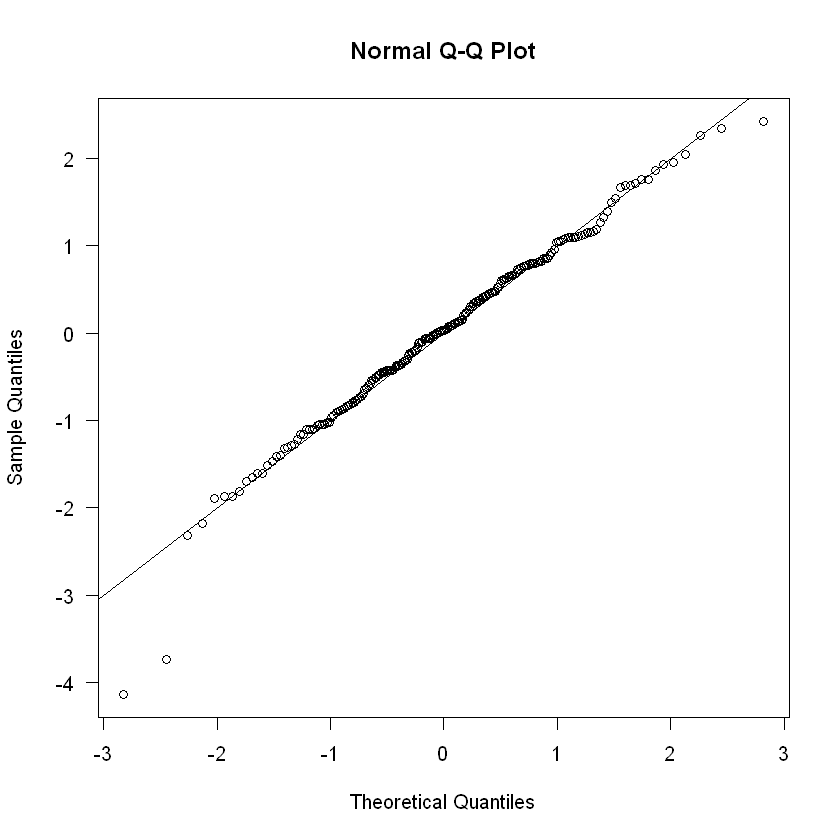
\includegraphics[width=\textwidth]{figures/minmax_mb_quantile_resid.png}
            \caption{Quantile residual của mô hình backward (dữ liệu được tiền xử lý minmax)}
        \end{subfigure}
        \hfill
        \begin{subfigure}[b]{0.4\textwidth}
            \centering
            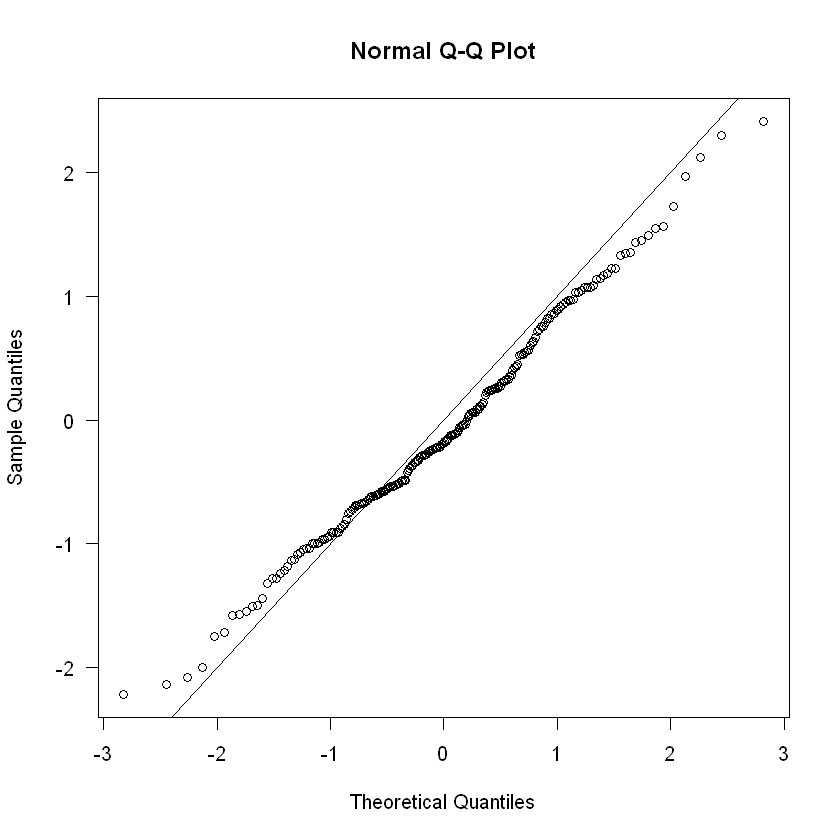
\includegraphics[width=\textwidth]{figures/standardize_mb_quantile_resid.png}
            \caption{Quantile residual của mô hình backward (dữ liệu được tiền xử lý standardize)}
        \end{subfigure}
        \caption{Quantile residual của mô hình backward}
        \label{fig:Quantile-resid-mb}
    \end{figure}

    Hình \ref{fig:Quantile-resid-mb} cho ta thấy đồ thị Q-Q plot của mô hình backward ứng với dữ liệu được tiền xử lý theo cách standardize không quá chuẩn.
    Ta nhận thấy mô hình gần như không thỏa mãn về điều kiện quantile residual phải có phân phối chuẩn tắc.


    \begin{figure}[h!]
        \centering
        \begin{subfigure}[b]{0.4\textwidth}
            \centering
            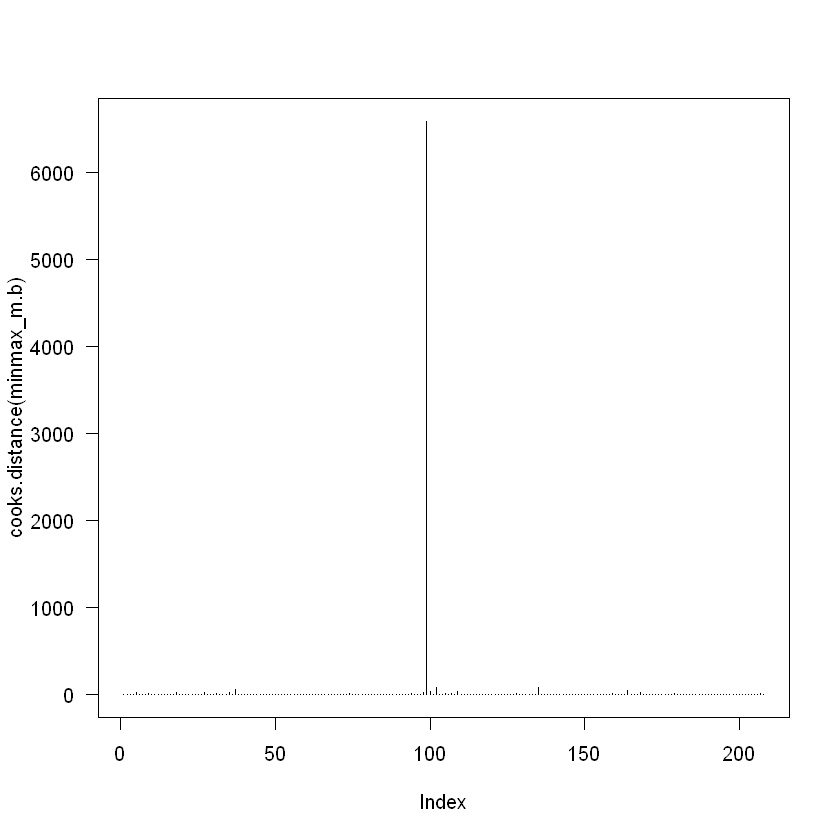
\includegraphics[width=\textwidth]{figures/minmax_mb_cooks.png}
            \caption{Cooks distance của mô hình backward (dữ liệu được tiền xử lý minmax)}
        \end{subfigure}
        \hfill
        \begin{subfigure}[b]{0.4\textwidth}
            \centering
            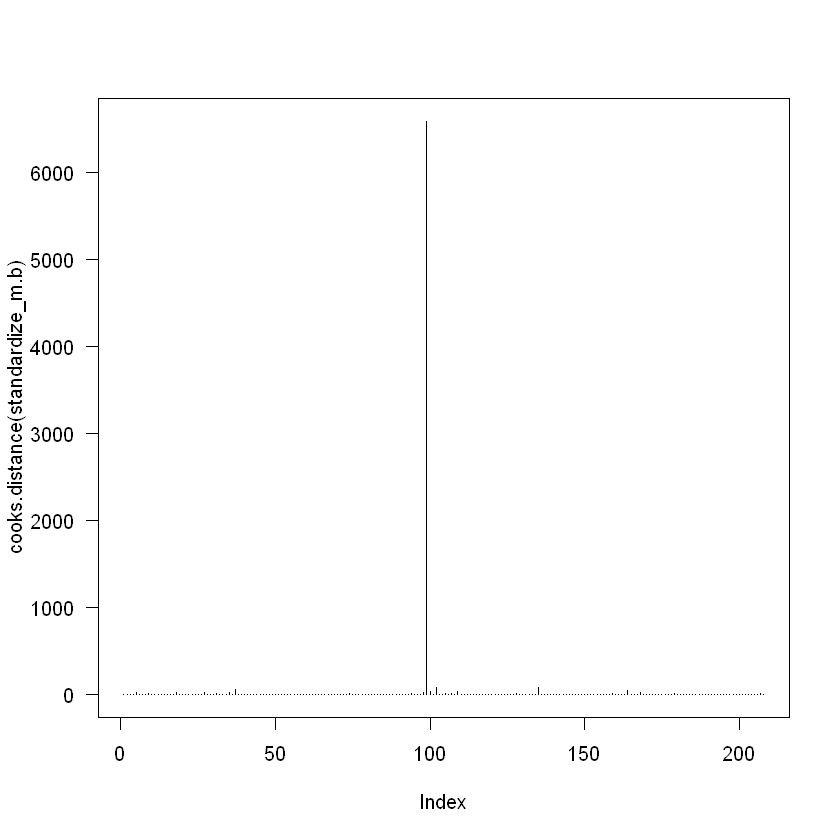
\includegraphics[width=\textwidth]{figures/standardize_mb_cooks.png}
            \caption{Cooks distance của mô hình backward (dữ liệu được tiền xử lý standardize)}
        \end{subfigure}
        \caption{Cooks distance của mô hình backward}
        \label{fig:Cooks-distance-mb}
    \end{figure}

    Hình \ref{fig:Cooks-distance-mb} cho ta thấy ví dụ học số 99 có giá trị Cooks distance quá lớn so với các ví dụ còn lại.

    \begin{figure}[h!]
        \centering
        \begin{subfigure}[b]{0.4\textwidth}
            \centering
            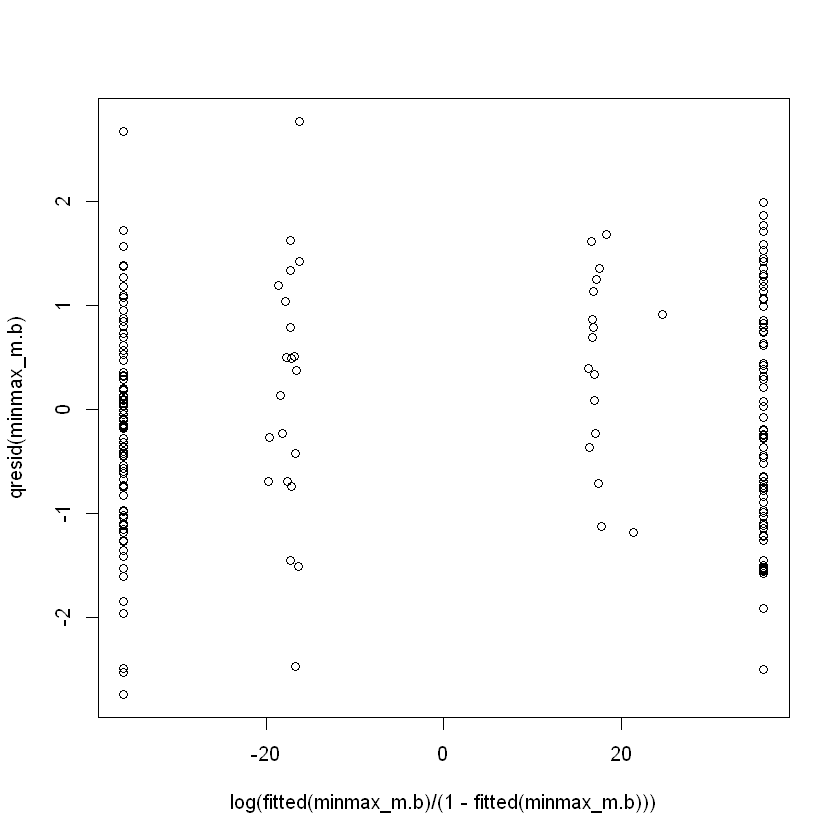
\includegraphics[width=\textwidth]{figures/minmax_mb_fitted.png}
            \caption{Quantile residual theo fitted value của mô hình backward (dữ liệu được tiền xử lý minmax)}
        \end{subfigure}
        \hfill
        \begin{subfigure}[b]{0.4\textwidth}
            \centering
            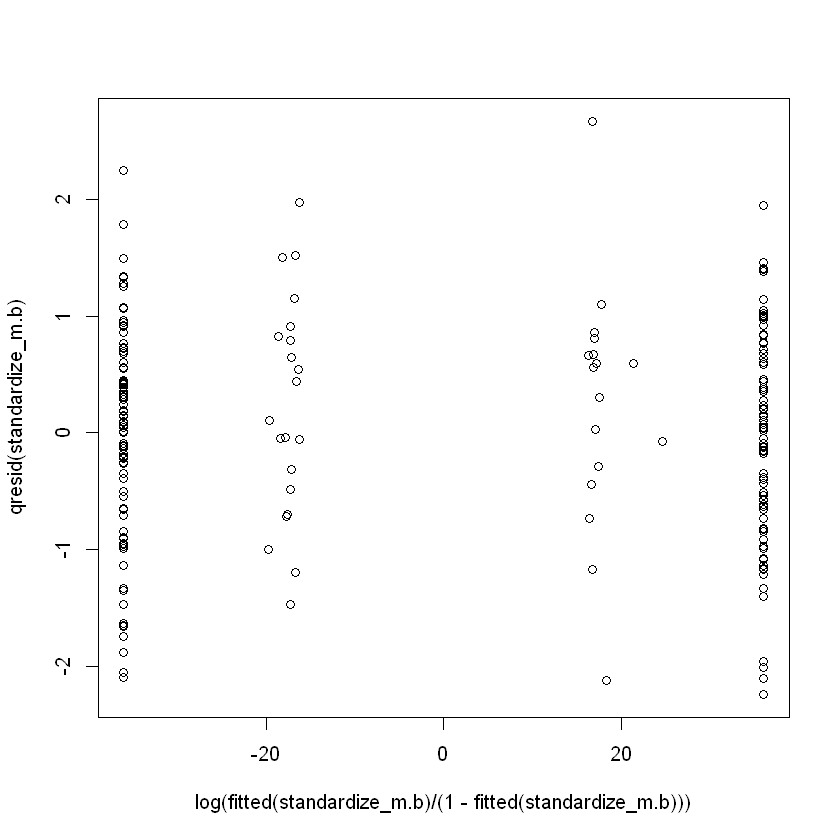
\includegraphics[width=\textwidth]{figures/standardize_mb_fitted.png}
            \caption{Quantile residual theo fitted value của mô hình backward (dữ liệu được tiền xử lý standardize)}
        \end{subfigure}
        \caption{Quantile residual theo fitted value của mô hình backward}
        \label{fig:Quantile-fitted-mb}
    \end{figure}

    Hình \ref{fig:Quantile-resid-mb} cho thấy mô hình backward các giá trị lại tập trung về hai phía của $\eta$ lý do là vì các tham số tương ứng với từng biến của mô hình backward quá lớn khiến cho giá trị $\eta$ được dùng để phân lớp quá rõ ràng trở nên rất lớn hoặc rất nhỏ.
    Các hệ số học được của mô hình backward:

    \begin{verbatim}
summary(minmax_m.b)
    \end{verbatim}

    \begin{verbatim}
        Coefficients:
        Estimate Std. Error z value Pr(>|z|)
(Intercept)     6357     472158   0.013    0.989
V1             -2919     331827  -0.009    0.993
V3              2744     398441   0.007    0.995
V7              1373     108270   0.013    0.990
V9             -1159      73803  -0.016    0.987
V12            -4601     156363  -0.029    0.977
V13             2275     105631   0.022    0.983
V14            -1929     122348  -0.016    0.987
V16             3245     357947   0.009    0.993
V17             2646     112430   0.024    0.981
V18            -4956     411919  -0.012    0.990
V19             2785     315026   0.009    0.993
V20            -6646     559139  -0.012    0.991
V21             6759     449049   0.015    0.988
V22            -8919     491708  -0.018    0.986
    \end{verbatim}

    Ta kiểm định các hệ số của mô hình forward-backward sử dụng likelihood ratio test:

    \begin{verbatim}
anova(minmax_m.bo, test="Chisq")
    \end{verbatim}
    
    \begin{verbatim}
Df	Deviance	Resid. Df	Resid. Dev	Pr(>Chi)
<int>	<dbl>	<int>	<dbl>	<dbl>
NULL	NA	NA	207	287.4062	NA
V2	1	12.3993380	206	275.0069	4.294861e-04
V4	1	7.2353306	205	267.7715	7.148265e-03
V10	1	17.6355013	204	250.1360	2.675471e-05
V11	1	14.7399471	203	235.3961	1.234037e-04
V17	1	7.1135689	202	228.2825	7.650265e-03
V20	1	7.9403408	201	220.3422	4.834473e-03
V21	1	2.6332555	200	217.7089	1.046469e-01
V22	1	3.4019489	199	214.3070	6.511944e-02
V29	1	4.6766949	198	209.6303	3.057452e-02
V30	1	0.1571336	197	209.4731	6.918094e-01
V31	1	2.8813646	196	206.5918	8.961005e-02
V32	1	5.0170651	195	201.5747	2.509867e-02
V34	1	11.6135724	194	189.9611	6.547227e-04
V35	1	1.1156477	193	188.8455	2.908575e-01
V36	1	10.0702347	192	178.7753	1.506838e-03
V49	1	27.9711885	191	150.8041	1.231352e-07
V50	1	5.2407937	190	145.5633	2.206321e-02        
    \end{verbatim}

    \begin{verbatim}
anova(standardize_m.bo, test="Chisq")
    \end{verbatim}

    \begin{verbatim}
Df	Deviance	Resid. Df	Resid. Dev	Pr(>Chi)
<int>	<dbl>	<int>	<dbl>	<dbl>
NULL	NA	NA	207	287.4062	NA
V2	1	12.3993380	206	275.0069	4.294861e-04
V4	1	7.2353306	205	267.7715	7.148265e-03
V10	1	17.6355013	204	250.1360	2.675471e-05
V11	1	14.7399471	203	235.3961	1.234037e-04
V17	1	7.1135689	202	228.2825	7.650265e-03
V20	1	7.9403408	201	220.3422	4.834473e-03
V21	1	2.6332555	200	217.7089	1.046469e-01
V22	1	3.4019489	199	214.3070	6.511944e-02
V29	1	4.6766949	198	209.6303	3.057452e-02
V30	1	0.1571336	197	209.4731	6.918094e-01
V31	1	2.8813646	196	206.5918	8.961005e-02
V32	1	5.0170651	195	201.5747	2.509867e-02
V34	1	11.6135724	194	189.9611	6.547227e-04
V35	1	1.1156477	193	188.8455	2.908575e-01
V36	1	10.0702347	192	178.7753	1.506838e-03
V49	1	27.9711885	191	150.8041	1.231352e-07
V50	1	5.2407937	190	145.5633	2.206321e-02
    \end{verbatim}

    Từ bảng phân tích phương sai, hầu hết các biến đầu đóng vai trò đáng kể trong mô hình ngoại trừ biến V21 và biến V35

    \begin{figure}[h!]
        \centering
        \begin{subfigure}[b]{0.4\textwidth}
            \centering
            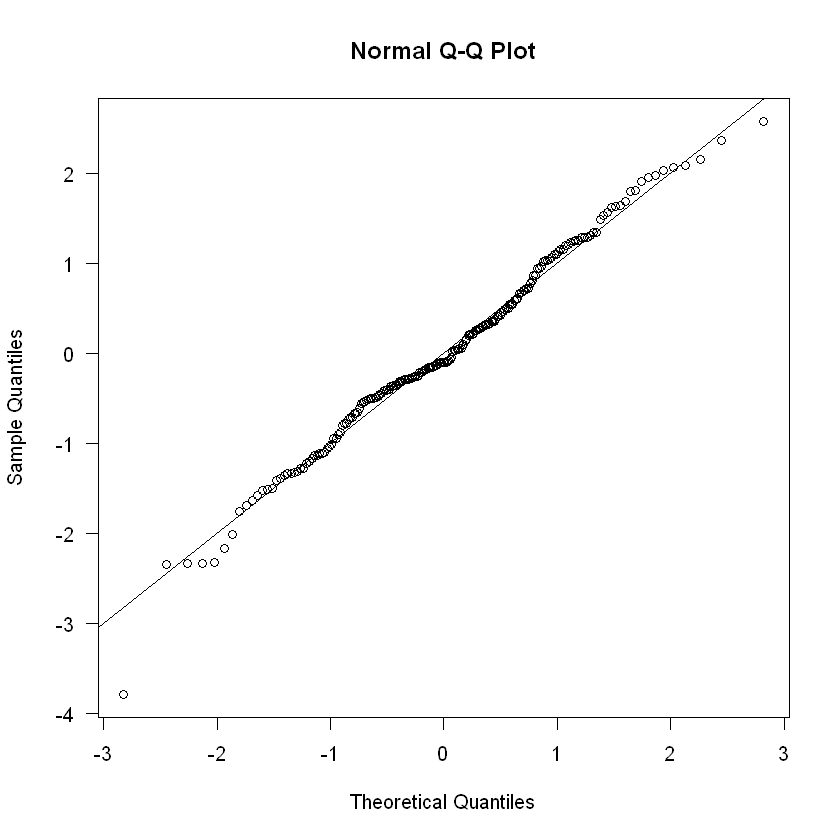
\includegraphics[width=\textwidth]{figures/minmax_mbo_quantile_resid.png}
            \caption{Quantile residual của mô hình forward-backward (dữ liệu được tiền xử lý minmax)}
        \end{subfigure}
        \hfill
        \begin{subfigure}[b]{0.4\textwidth}
            \centering
            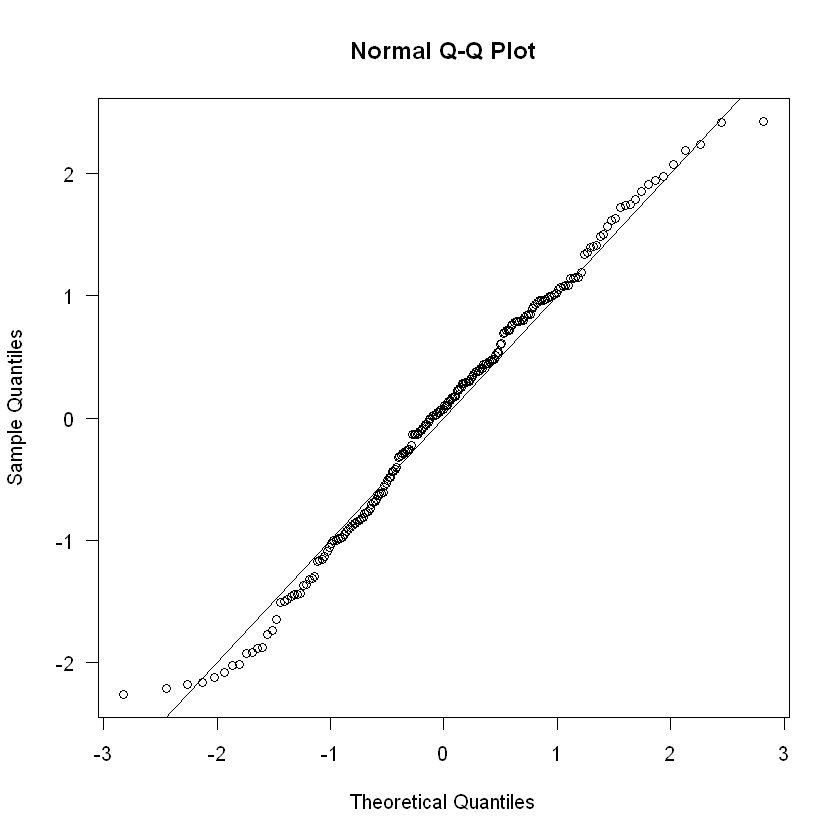
\includegraphics[width=\textwidth]{figures/standardize_mbo_quantile_resid.png}
            \caption{Quantile residual của mô hình forward-backward (dữ liệu được tiền xử lý standardize)}
        \end{subfigure}
        \caption{Quantile residual của mô hình forward-backward}
        \label{fig:Quantile-resid-mbo}
    \end{figure}

    Hình \ref{fig:Quantile-fitted-mbo} là đồ thị Q-Q plot của mô hình forward-backward cho thấy quantile residual có phân phối gần với phân phối chuẩn tắc.
    Mô hình forward-backward thỏa mãn giả thiết về quantile residual phải có phân phối chuẩn tắc.

    \begin{figure}[h!]
        \centering
        \begin{subfigure}[b]{0.4\textwidth}
            \centering
            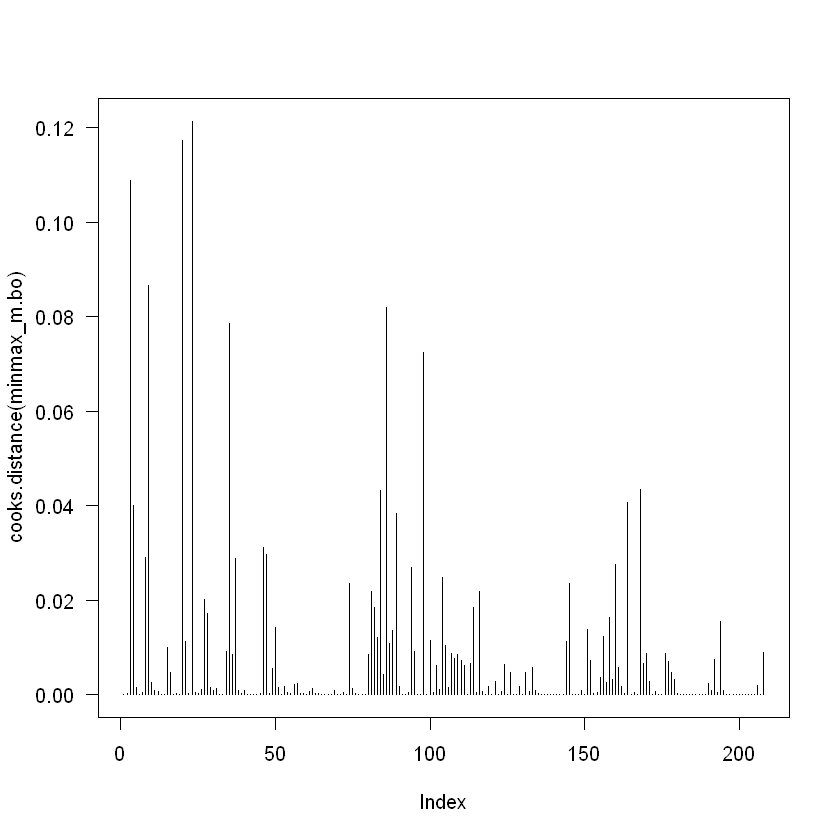
\includegraphics[width=\textwidth]{figures/minmax_mbo_cooks.png}
            \caption{Cooks distance của mô hình forward-backward (dữ liệu được tiền xử lý minmax)}
        \end{subfigure}
        \hfill
        \begin{subfigure}[b]{0.4\textwidth}
            \centering
            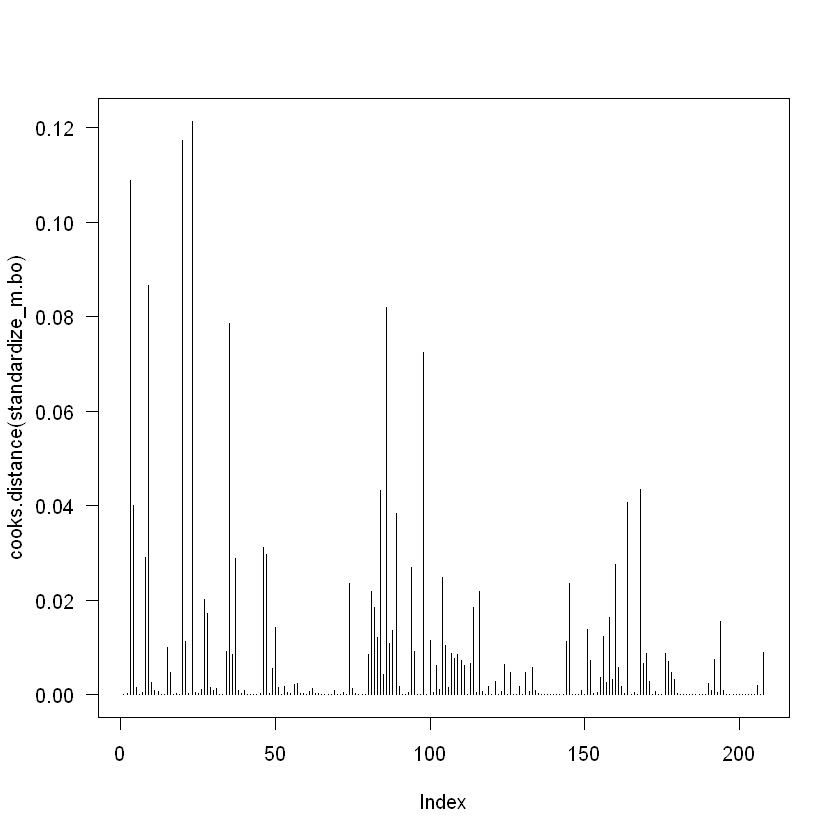
\includegraphics[width=\textwidth]{figures/standardize_mbo_cooks.png}
            \caption{Cooks distance của mô hình forward-backward (dữ liệu được tiền xử lý standardize)}
        \end{subfigure}
        \caption{Cooks distance của mô hình forward-backward}
        \label{fig:Cooks-distance-mbo}
    \end{figure}

    Hình \ref{fig:Quantile-fitted-mbo} cho thấy các giá trị Cooks distance của các ví dụ học khá nhỏ, lớn nhất bằng khoảng 0.12 trong khi phân vị mức F(0.5, 18, 208-18) có giá trị khoảng 0.9666.
    Như vậy mô hình forward-backward thỏa mãn về giả thiết không có điểm ngoại lai.

    \begin{figure}[h!]
        \centering
        \begin{subfigure}[b]{0.4\textwidth}
            \centering
            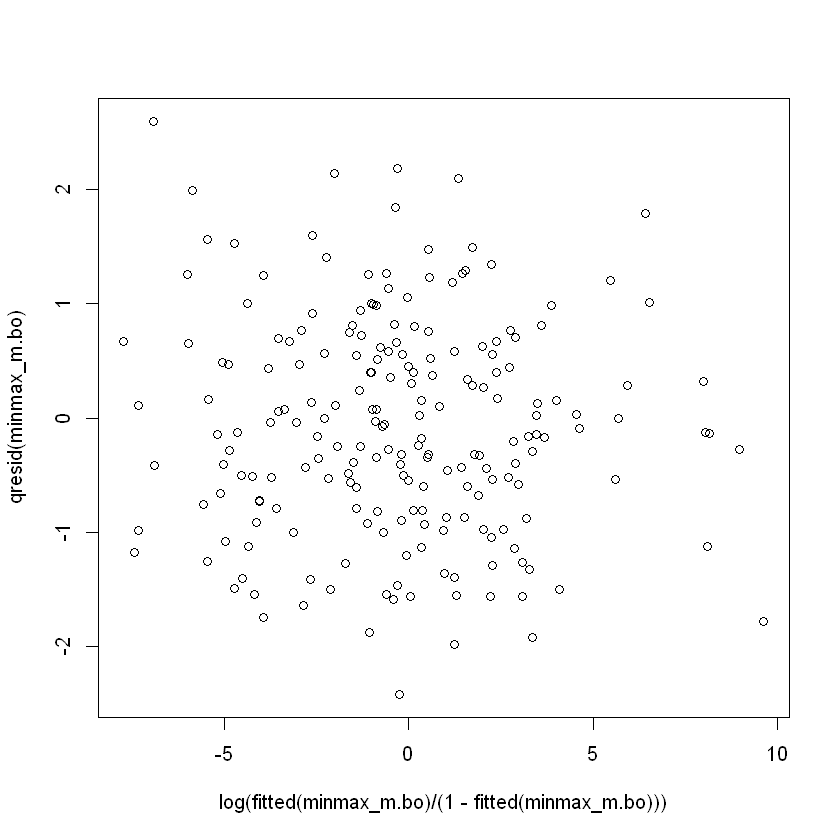
\includegraphics[width=\textwidth]{figures/minmax_mbo_fitted.png}
            \caption{Quantile residual theo fitted value của mô hình forward-backward (dữ liệu được tiền xử lý minmax)}
        \end{subfigure}
        \hfill
        \begin{subfigure}[b]{0.4\textwidth}
            \centering
            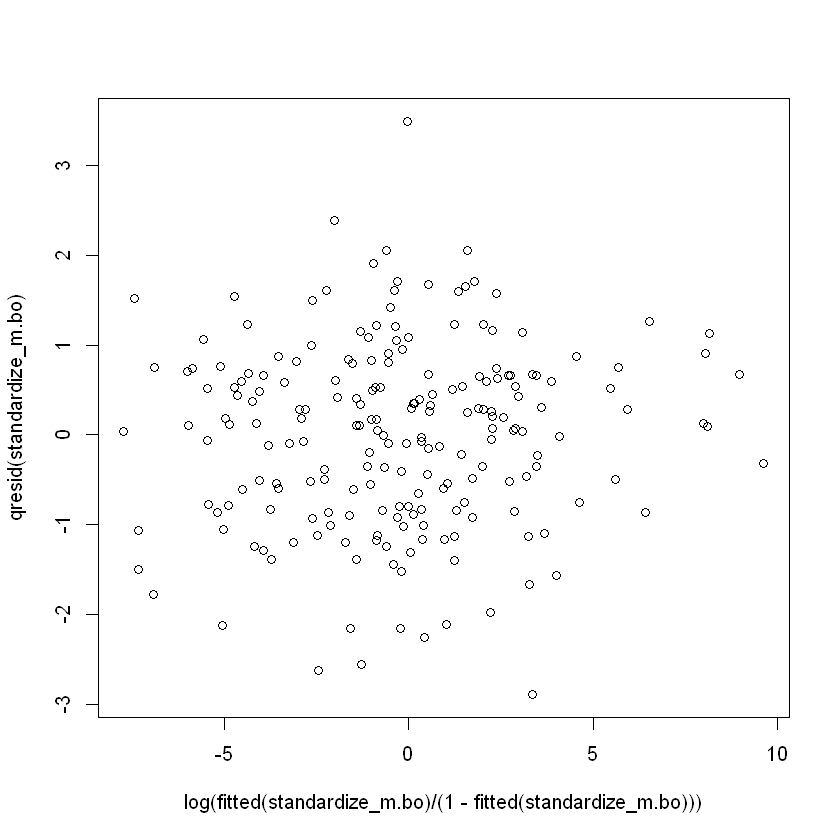
\includegraphics[width=\textwidth]{figures/standardize_mbo_fitted.png}
            \caption{Quantile residual theo fitted value của mô hình forward-backward (dữ liệu được tiền xử lý standardize)}
        \end{subfigure}
        \caption{Quantile residual theo fitted value của mô hình forward-backward}
        \label{fig:Quantile-fitted-mbo}
    \end{figure}

    Từ hình \ref{fig:Quantile-fitted-mbo} ta thấy mô hình forward-backward thể hiện khá tốt các giả định lý
    thuyết khi mà quantile residual ngẫu nhiên xung quanh điểm 0 và so với giá trị $\eta$ (log-odd) của mô
    hình cho thấy các ví dụ độc lập với nhau.

    Tổng hợp lại sử dụng 5 mô hình:

    \begin{itemize}
        \item Mô hình gồm tất cả các biến (ký hiệu là full)
        \item Mô hình forward được chọn ở trên (ký hiệu là m.f)
        \item Mô hình backward được chọn ở trên (ký hiệu là m.b)
        \item Mô hình forward-backward được chọn ở trên (ký hiệu là m.bo)
        \item Mô hình các biến được trích xuất từ thuật toán PCA giữ lại 95 \% thông tin (ký hiệu là pca\_x với x là thuật toán PCA giữ lại x \% thông tin)
    \end{itemize}

    Để chọn ra mô hình tốt nhất, mỗi mô hình đi kèm với cách hiệu chỉnh sẽ được tối ưu hóa các siêu tham số gồm:

    \begin{itemize}
        \item Phương pháp tiền xử lý: min-max scaling, standardize.
        \item Tốc độ học được biến đổi trong quá trình huấn luyện theo các cách: fixed, cyclic, inverse\_decay, exponential\_decay, factor\_decay, squareroot, cosine.
        \item Các tốc độ học khác nhau: 1e-4, 1e-3, 1e-2, 1e-1, 1, 2, 5, 10
        \item Các thuật toán tối ưu hóa, 12 thuật toán tối ưu hóa được sử dụng gồm:
        \begin{itemize}
            \item Gradient Descent
            \item Adam
            \item Avagrad
            \item RAdam
            \item Momentum
            \item Adagrad
            \item RMSProp
            \item Adadelta
            \item Adamax
            \item Nadam
            \item AMSGrad
            \item AdaBelief
        \end{itemize}

        Sơ đồ mã giả của các thuật toán tối ưu hóa được trình bày ở phụ lục \ref{Optimization-Algorithms} và chi tiết các phương pháp điều chỉnh tốc độ học được trình bày ở phục lục \ref{LRScheduler}
    \end{itemize}

    Các siêu tham số trên sẽ được huấn luyện sử dụng code python và numpy không sử dụng thư viện khác.
    Việc sử dụng code python và numpy để có thể thử với các thuật toán tối ưu hóa khác mà thư viện sklearn không có.
    Hệ số $\lambda$ trong quá trình huấn luyện các mô hình được tự cài đặt bằng python và numpy được cố định là 1e-3 (do hạn chế về mặt thời gian).
    Kết quả của quá trình tối ưu hóa siêu tham số cho các mô hình được cài đặt bằng python và numpy được trình bày ở bảng \ref{tab:custom-hyperparameter-result} với cột bên trái ngoài cùng là loại mô hình (được hình thành từ các biến giải thích sử dụng và phương pháp hiệu chỉnh) các cột bên phải là tổ hợp các siêu tham số tối ưu tương ứng.

    Ngoài ra ta vẫn huấn luyện một tập các mô hình được huấn luyện sử dụng thư viện sklearn.
    Vì vấn đề thời gian đối với các mô hình được huấn luyện trên sklearn chỉ gồm 3 mô hình:
    \begin{itemize}
        \item Mô hình gồm tất cả các biến
        \item Mô hình forward-backward
        \item Mô hình các biến được trích xuất từ thuật toán PCA giữ lại 95 \% thông tin
    \end{itemize}
    Siêu tham số của các mô hình được huấn luyện sử dụng sklearn bao gồm:

    \begin{itemize}
        \item Phương pháp tiền xử lý: min-max scaling, standardize.
        \item Các hệ số $C$ là nghịch đảo của $\lambda$
        \item Các thuật toán tối ưu hóa, 6 thuật toán tối ưu hóa được sử dụng gồm:
        \begin{itemize}
            \item lbfgs
            \item liblinear
            \item newton-cg 
            \item newton-cholesky
            \item sag 
            \item saga
        \end{itemize}
    \end{itemize}

    Phương pháp hiệu chỉnh "l1" được gọi là Lasso, phương pháp hiệu chỉnh "l2" được gọi là Ridge, không hiệu chỉnh ta gọi là Naive
    Mỗi một cặp thông tin gồm phương pháp hiệu chỉnh ("l1", "l2", không hiệu chỉnh) và mô hình sẽ được chọn ra bộ siêu tham số tốt nhất từ các siêu tham số được đề cập ở trên bằng độ đo AUC-ROC trên tập test.
    Ta sẽ cố định tập test ngay từ đầu.
    Như vậy ta sẽ có 5 (mô hình) $\times$ 3 ("l1"-lasso, "l2"-ridge, không hiệu chỉnh) = 15 mô hình ứng viên được cài đặt bằng ngôn ngữ python và numpy được chọn từ quá trình tối ưu hóa siêu tham số và 9 mô hình ứng viên được huấn luyện bằng thư viện sklearn.
    Như vậy ta có 24 mô hình ứng viên.

    Từ các mô hình ứng viên, để chọn ra mô hình tốt nhất từ nhiều yếu tố như $AUC-ROC, AIC, BIC$ cũng như từ trung bình hình học G-Means giữa độ nhạy (Sensitivity) và độ đặc hiệu (Specificity) ứng với ngưỡng xác suất $p^*$ ($p^*$ làm cho G-Means cực đại) được chọn.

    \begin{table}[h!]
        \centering
        \begin{tabular}{|c | c | c | c | c |}
            \hline
            Mô hình & Phương pháp chuẩn hóa & Thuật toán tối ưu & Scheduler & Init learning rate \\
            \hline
            \hline
            full - Naive & standardize & RMSProp & inverse decay & 5 \\
            \hline
            m.bo - Naive & standardize & AdaBelief & fixed & 5 \\
            \hline
            m.f - Naive & standardize & RMSProp & squareroot &5 \\
            \hline
            m.b - Naive & standardize & RMSProp & cosine & 1 \\
            \hline
            pca\_95 - Naive & standardize & Gradient\_Descent & inverse\_decay & 10 \\
            \hline
            full - Lasso & minmax & Avagrad & squareroot & 10 \\
            \hline
            m.bo - Lasso & standardize & Adam & exponential\_decay & 10 \\
            \hline
            m.f - Lasso & standardize & RMSProp & fixed &2 \\
            \hline
            m.b - Lasso & standardize & AMSGrad & cyclic & 5 \\
            \hline
            pca\_95 - Lasso & standardize & Gradient\_Descent & cosine & 0.01 \\
            \hline
            full - Ridge & standardize & RAdam & fixed & 10 \\
            \hline
            m.bo - Ridge & standardize & Adam & fixed & 5 \\
            \hline
            m.f - Ridge & standardize & RAdam & fixed & 10 \\
            \hline
            m.b - Ridge & standardize & RAdam & fixed & 10 \\
            \hline
            pca\_95 - Ridge & standardize & RAdam & fixed & 10 \\
            \hline
        \end{tabular}
        \caption{Các siêu tham số tốt nhất với từng mô hình (mỗi mô hình được xác định bằng các biến \\ giải thích và phương pháp hiệu chỉnh (naive, ridge, lasso))}
        \label{tab:custom-hyperparameter-result}
    \end{table}


    \begin{table}[h!]
        \centering
        \begin{tabular}{|c | c | c | c | c |}
            \hline
            Mô hình & Random\_state & Phương pháp chuẩn hóa & Thuật toán tối ưu & C \\
            \hline
            \hline
            Sklearn full - Naive & 379 & minmax & sag & 0.0001 \\
            \hline
            Sklearn m.bo - Naive & 953 & standardize & sag & 0.0001 \\
            \hline
            Sklearn pca\_95 - Naive & 431 & minmax & sag & 0.0001 \\
            \hline
            Sklearn full - Lasso & 587 & standardize & saga & 1000 \\
            \hline
            Sklearn m.bo - Lasso & 0 & standardize & liblinear & 10 \\
            \hline
            Sklearn pca\_95 - Lasso & 2 & minmax & saga & 0.1 \\
            \hline
            Sklearn full - Ridge & 0 & minmax & lbfgs & 10 \\
            \hline
            Sklearn m.bo - Ridge & 85 & standardize & sag & 100 \\
            \hline
            Sklearn pca\_95 - Ridge & 0 & minmax & lbfgs & 10 \\
            \hline
        \end{tabular}
        \caption{Các siêu tham số tốt nhất với từng mô hình được huấn luyện sử dụng thư viện sklearn (mỗi mô hình được xác định bằng các biến giải thích và phương pháp hiệu chỉnh (naive, ridge, lasso))}
        \label{tab:sklearn-hyperparameter-result}
    \end{table}

    Random\_state được chính là seed để khởi tạo các tham số của mô hình.
    Còn tập dữ liệu được chia tập train và tập test một cách cố định từ ban đầu (sử dụng random\_state 42)

    Kết quả của quá trình tối ưu hóa siêu tham số cho các mô hình được cài đặt bằng python và numpy được trình bày ở bảng \ref{tab:custom-hyperparameter-result}.
    Kết quả của quá trình tối ưu hóa siêu tham số cho các mô hình được cài đặt bằng sklearn được trình bày ở bảng \ref{tab:sklearn-hyperparameter-result}

    Để chọn ra ngưỡng xác suất $p^*$ tốt nhất với từng mô hình ta tìm ngưỡng xác suất sao cho cực đại hóa trung bình hình học giữa độ nhạy (Sensitivity) và độ đặc hiệu (Specificity).
    Ta có công thức tính các đại lượng trên:

    \begin{equation*}
        \begin{aligned}
            \mathrm{TPR} = \mathrm{Precision} = \mathrm{Sensitivity} &= \dfrac{\mathrm{TP}}{\mathrm{TP} + \mathrm{FN}} \\
            \mathrm{FPR} &= \dfrac{\mathrm{FP}}{\mathrm{FP} + \mathrm{TN}} \\
            \mathrm{Specificity} = 1 - \mathrm{FPR} &= \dfrac{\mathrm{TN}}{\mathrm{FP} + \mathrm{TN}}
        \end{aligned}
    \end{equation*}

    Trung bình hình học giữa giữa độ nhạy (Sensitivity) và độ đặc hiệu (Specificity) là:
    \begin{equation*}
        \mathrm{G-Means} = \sqrt{\mathrm{Sensitivity} \times \mathrm{Specificity}} = \sqrt{\dfrac{\mathrm{TP}}{\mathrm{TP} + \mathrm{FN}} \times \dfrac{\mathrm{TN}}{\mathrm{FP} + \mathrm{TN}}}
    \end{equation*}

    Như ta đã biết đường cong ROC được xây dựng bằng cách chọn các ngưỡng xác suất $p$ để một mẫu được phân loại thành nhãn 1 hay nhãn 0 (mẫu được xem là nhãn 1 nếukết quả đầu ra lớn hơn 1 và ngược lại được xem là nhãn 0).
    Như vậy với mỗi ngưỡng xác suất sẽ có một bảng ma trận nhầm lẫn khác nhau (TP, TN, FP, FN thay đổi dựa theo ngưỡng xác suất) hay sẽ có các giá trị độ nhạy (Sensitivity) và độ đặc hiệu (Specificity) khác nhau từ đó dẫn đến trung bình hình học G-Means giữa hai đại lượng này cũng thay đổi.
    Ta chọn $p^*$ sao cho làm cực đại hóa giá trị G-Means:

    \begin{equation*}
        p^* = \underset{p}{\mathrm{argmax}} \mathrm{G-Means} = \underset{p}{\mathrm{argmax}} \sqrt{\mathrm{Sensitivity} \times \mathrm{Specificity}} = \underset{p}{\mathrm{argmax}} \sqrt{\dfrac{\mathrm{TP}}{\mathrm{TP} + \mathrm{FN}} \times \dfrac{\mathrm{TN}}{\mathrm{FP} + \mathrm{TN}}}
    \end{equation*}

    Để tính giá trị $p^*$ ta sử dụng đoạn code sau:

    \begin{python}
y_pred = model.predict(x=test_x, return_prob=True)
fpr, tpr, thresholds = roc_curve(y_true=test_y, y_score=y_pred)
area_roc = auc(fpr, tpr)
gmeans = compute_gmeans(tpr=tpr, fpr=fpr)
        
idx = np.argmax(gmeans)
prob_star = thresholds[idx]
gmean_star = gmeans[idx]
    \end{python}

    Ta sẽ lựa chọn mô hình dựa trên nhiều tiêu chí:

    \begin{itemize}
        \item AUC-ROC
        \item G-Means
        \item AIC
        \item BIC
    \end{itemize}

    Công thức của BIC:

    \begin{equation*}
        BIC = -2 \log L + p\log n
    \end{equation*}

    với $p$ là số biến giải thích trong mô hình, $L$ là ước lượng hợp lý của mô hình, $n$ là số ví dụ của tập dữ liệu.

    Trong mô hình logistic, ước lượng hợp lý bởi công thức:

    \begin{equation*}
        L = \prod_{i=1}^n p_i^{y_i}(1-p_i)^{1 - y_i}
    \end{equation*}

    với $p_i$ là xác suất đầu ra của mô hình với đầu vào là ví dụ thứ $i$ trong tập dữ liệu, $y_i$ là nhãn của dữ liệu thứ $i$.

    Các đại lượng AIC, BIC tổng hòa khả năng giải thích của mô hình và có phạt độ phức tạp của mô hình (AIC chỉ phạt theo số biến giải thích, BIC phạt theo cả số biến giải thích và số ví dụ trong tập dữ liệu).

    \begin{figure}[h!]
        \centering
        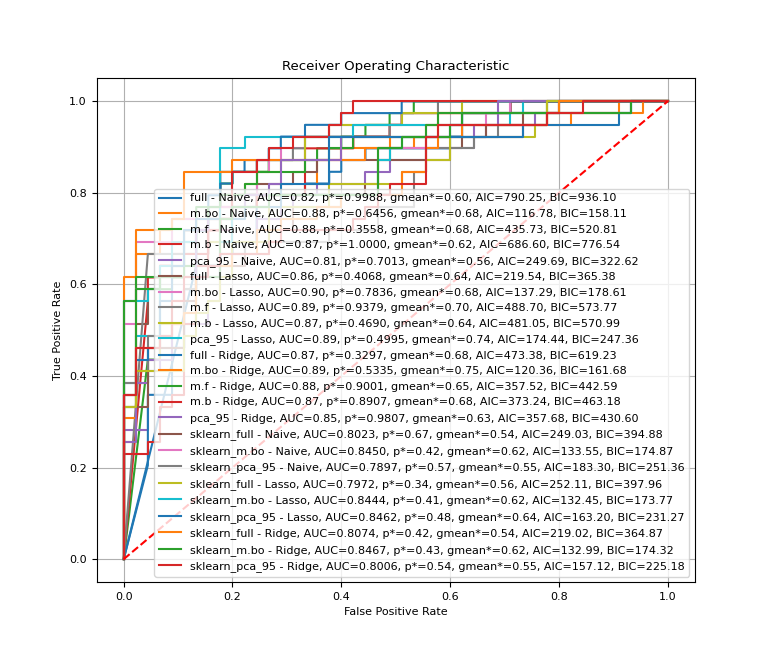
\includegraphics[width=1.0\textwidth]{figures/roc_curve_summary.png}
        \caption{Tổng hợp kết quả các mô hình}
        \label{fig:roc-curve-summary}
    \end{figure}

    Hình \ref{fig:roc-curve-summary} tổng hợp kết quả của các mô hình gồm có thông tin về AUC-ROC, các thông số như AIC, BIC.
    Các mô hình có tiền tố "Sklearn" có ý nghĩa rằng mô hình được huấn luyện sử dụng thư viện sklearn để phân biệt với các mô hình được cài đặt bằng python và numpy.
    Để tìm ngưỡng xác suất tối ưu để phân lớp ta sử dụng trung bình hình học của độ nhạy (Sensitivity) và độ đặc hiệu (Specificity).

    Ta nhận thấy một số mô hình có cả kết quả về G-Means cực đại, AUC-ROC và chỉ số AIC đều tốt như:

    \begin{itemize}
        \item m.bo-Ridge với $p^*=0.5335$, AUC = 0.89, G-Means = 0.75, AIC = 120.36, BIC = 161.68
        \item m.bo-Naive với $p^*=0.6456$, AUC = 0.88, G-Means = 0.68, AIC = 116.78, BIC = 158.11
        \item m.bo-Lasso với $p^*= 0.7836$, AUC = 0.90, G-Means = 0.68, AIC = 137.29, BIC = 178.61
        \item pca\_95-Lasso với $p^*= 0.4995$, AUC = 0.89, G-Means = 0.74, AIC = 174.44, BIC = 247.36
        \item Sklearn-m.bo-Lasso với $p^*= 0.4139$, AUC = 0.84, G-Means = 0.62, AIC = 132.45, BIC = 173.77
        \item Sklearn-m.bo-Ridge với $p^*= 0.4356$, AUC = 0.85, G-Means = 0.62, AIC = 132.99, BIC = 174.32
    \end{itemize}

    \begin{figure}[h!]
        \centering
        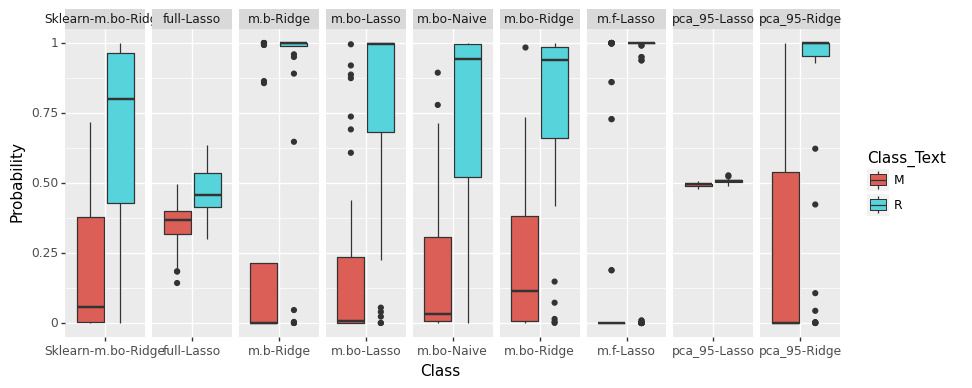
\includegraphics[width=1.0\textwidth]{figures/prob_box_plot.png}
        \caption{So sánh kết quả đầu ra của một số mô hình dùng box plot}
        \label{fig:prob-box-plot}
    \end{figure}

    Hình \ref{fig:prob-box-plot} vẽ box plot so sánh các kết quả đầu ra với từng mô hình.
    Ta nhận thấy mô hình pca\_95-Lasso dù có các chỉ số về AUC-ROC và G-Means rất tốt nhưng phân phối kết quả đầu ra của các ví dụ nhãn "M" và "R" rất sát nhau.
    Mặt khác ta thấy mô hình m.bo-Ridge và m.bo-Lasso có phân phối kết quả đầu ra tách biệt nhau khá lớn giữa hai lớp "M" và "R", ta thấy hai mô hình này về mặt trực quan có khả năng phân loại tốt nhất trong các mô hình trên.

    Ta kiểm tra các trọng số thu được của mô hình pca\_95-Lasso:

    \begin{verbatim}
[ 0.          0.00581896 -0.0134918   0.          0.          0.
0.          0.          0.          0.          0.          0.
0.          0.          0.          0.          0.          0.
0.          0.          0.          0.          0.          0.
0.          0.          0.          0.          0.          0.]
    \end{verbatim}

    Ta thấy các trọng số học được của mô hình pca\_95-Lasso rất thưa chỉ có 2 trọng số khác không nhưng cũng rất nhỏ.
    Điều này làm cho khác biệt về kết quả đầu ra giữa các nhãn nhỏ không đủ khoảng cách an toàn với những dữ liệu mới chưa gặp.

    Ta sẽ xét thêm ma trận nhầm lẫn (confusion matrix) của các mô hình trên tại ngưỡng xác suất $p^*$ đã được tính:

    \begin{verbatim}
m.bo-Ridge:    precision    recall  f1-score   support

        0       0.85      0.89      0.87        45
        1       0.86      0.82      0.84        39

 accuracy                           0.86        84
macro avg       0.86      0.85      0.86        84
weighted avg    0.86      0.86      0.86        84

m.bo-Naive:    precision    recall  f1-score   support

        0       0.79      0.91      0.85        45
        1       0.88      0.72      0.79        39

 accuracy                           0.82        84
macro avg       0.83      0.81      0.82        84
weighted avg    0.83      0.82      0.82        84

m.bo-Lasso:   precision    recall  f1-score   support

        0       0.79      0.91      0.85        45
        1       0.88      0.72      0.79        39

 accuracy                           0.82        84
macro avg       0.83      0.81      0.82        84
weighted avg    0.83      0.82      0.82        84

pca_95-Lasso:  precision  recall  f1-score   support

        0       0.88      0.82      0.85        45
        1       0.81      0.87      0.84        39

 accuracy                           0.85        84
macro avg       0.85      0.85      0.85        84
weighted avg    0.85      0.85      0.85        84

Sklearn-m.bo-Lasso:  precision    recall  f1-score   support

        0       0.78      0.80      0.79        45
        1       0.76      0.74      0.75        39

 accuracy                           0.77        84
macro avg       0.77      0.77      0.77        84
weighted avg    0.77      0.77      0.77        84

Sklearn-m.bo-Ridge: precision    recall  f1-score   support

        0       0.78      0.80      0.79        45
        1       0.76      0.74      0.75        39

 accuracy                           0.77        84
macro avg       0.77      0.77      0.77        84
weighted avg    0.77      0.77      0.77        84

    \end{verbatim}

    \begin{figure}[h!]
        \centering
        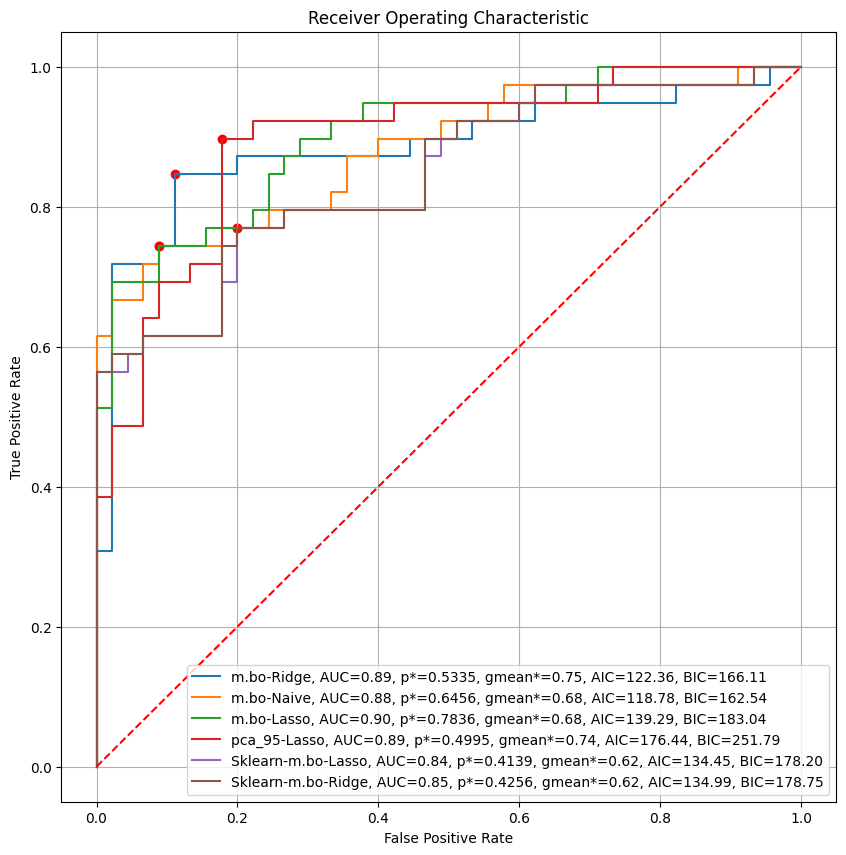
\includegraphics[width=1.0\textwidth]{figures/little_roc_curve_summary.png}
        \caption{Tổng hợp kết quả các mô hình có kết quả tốt nhất. Dấu chấm đỏ thể hiện điểm ($\mathrm{FPR}^*, \mathrm{TPR}^*$) tương ứng với ngưỡng $p^*$ làm cực đại G-Means}
        \label{fig:little-roc-curve-summary}
    \end{figure}

    Từ hình \ref{fig:little-roc-curve-summary} và các ma trận nhầm lẫn của các mô hình tại ngưỡng xác suất $p^*$ đã được tính thì hai mô hình m.bo-Ridge và mô hình pca\_95-Lasso có kết quả tốt nhất (Precision, Recall, F1-score cao nhất) nhưng như ở trên ta đã thấy không có sự tách biệt lớn về phân phối đầu ra giữa các nhãn của mô hình pca\_95-Lasso nên quyết định cuối cùng ta chọn mô hình m.bo-Ridge

    Ở bài tập 2 (tuần thứ 3), mỗi mô hình trên được tối ưu hóa siêu tham số theo hai cách:

    \begin{itemize}
        \item Chỉ tối ưu trên random\_state của mô hình logistic (cách khởi tạo mô hình).
        \item Tối ưu trên các siêu tham số random\_state, C, solver, regularization (l1, l2, elasticnet).
    \end{itemize}

    \begin{figure}[h!]
        \centering
        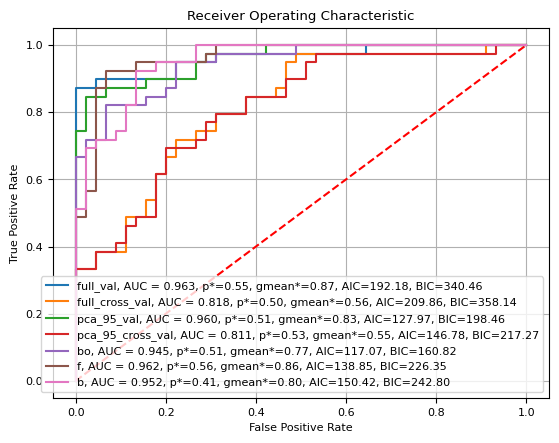
\includegraphics[width=1.0\textwidth]{figures/ROC_Curve_AIC_BIC_Excercise_2_1.png}
        \caption{ So sánh đường cong ROC, $p^*$, G-Means tương ứng với $p^*$, chỉ số AIC, BIC của các mô hình được tối ưu hóa tham số ở bài tập 2 theo cách 1}
        \label{fig:ROC-Curve-AIC-BIC_Excercise-2-1}
    \end{figure}

    \begin{figure}[h!]
        \centering
        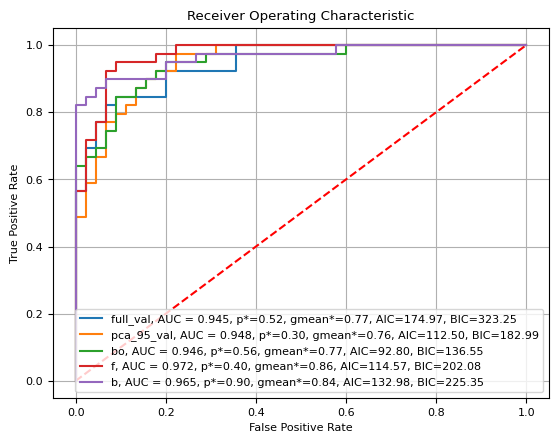
\includegraphics[width=1.0\textwidth]{figures/ROC_Curve_AIC_BIC_Excercise_2_2.png}
        \caption{ So sánh đường cong ROC, $p^*$, G-Means tương ứng với $p^*$, chỉ số AIC, BIC của các mô hình được tối ưu hóa tham số ở bài tập 2 theo cách 2}
        \label{fig:ROC-Curve-AIC-BIC_Excercise-2-2}
    \end{figure}

    Ở bài tập số 2 (tuần số 3), với mỗi mô hình ta đã chạy tối ưu hóa tham số trong đó các phương pháp hiệu chỉnh như Ridge, Lasso, Elasticnet đã được sử dụng.
    Hình \ref{fig:ROC-Curve-AIC-BIC_Excercise-2-1} và \ref{fig:ROC-Curve-AIC-BIC_Excercise-2-2} tổng hợp đường cong ROC, $p^*$, G-Means tương ứng với $p^*$, chỉ số AIC, BIC của các mô hình được tối ưu hóa tham số ở bài tập 2.
    Ta nhận thấy kết quả các mô hình ở bài tập trước cho kết quả cao hơn thế nhưng trong các mô hình ở bài tập trước việc chia tập train và test khác nhau có thể dẫn đến những tập test có các ví dụ điển hình của các lớp làm cho các thông số như AUC-ROC, G-Means cực đại cao lên.
    Còn ở bài tập số 3, ta cố định trước tập train và tập test cho mọi mô hình và kiểm tra mô hình trên tập test cố định này.
\end{loigiai}

\newpage
    \section*{Kết luận}
    Ta chọn mô hình forward-backward m.bo-Ridge với ngưỡng $p^*=0.5335$, AUC = 0.89, G-Means = 0.75, AIC = 120.36, BIC = 161.68.
    Do những hạn chế về thời gian nên bài tập chưa thể chạy tối ưu thêm một số các siêu tham số ở các mô hình tự cài đặt bằng python và numpy như hệ số $\lambda$ (hệ số $\lambda$ được tối ưu hóa trong huấn luyện các mô hình bằng sklearn nhưng trong các mô hình tự cài đặt $\lambda$ được đặt bằng 1e-3).
    Mô hình forward-backward cho kết quả tốt nhất dù theo Naive, Lasso hay Ridge lý do là vì đã được trích chọn đặc trưng từ quá trình chọn các đặc trưng sao cho cực đại hóa ước lượng hợp lý trên dữ liệu.
    Ngoài ra phương pháp phân tích thành phần chính PCA cũng cho kết quả khá tốt do PCA đã trích xuất ra các đặc trưng độc lập dẫn đến làm giảm sự đa cộng tuyến trong mô hình.
    Các mô hình sử dụng phương pháp hiệu chỉnh Lasso thường cho các trọng số khá thưa (nhiều trọng số là 0), một số mô hình cho kết quả phân loại trên tập test khá tốt nhưng do nhiều trọng số bằng 0 cũng như các trọng số khác 0 vẫn có trị tuyệt đối nhỏ làm cho các mô hình này không có ranh giới lớn về phân phối đầu ra giữa các nhãn.
\newpage
\printbibliography[title={TÀI LIỆU THAM KHẢO}]

\newpage
\appendix

\section{Các thuật toán tối ưu hóa} \label{Optimization-Algorithms}


\begin{algorithm}[h!]
    \DontPrintSemicolon
    \KwIn{độ dài bước $\lbrace \alpha_t \rbrace_{t=1}^{T}$, $w_0$ khởi tạo, hàm mục tiêu $\ell(w)$}
    \KwOut{$w$ đã được học}

    \For{$t \gets 1$ \KwSty{to} $T$} {
        $g_t \gets \nabla \ell(w_{t-1})$\;
        $w_t \gets w_{t-1} - \alpha_t g_t$
    }
    \Return{$w_T$}\;
    \caption{Thuật toán Gradient Descent}
\end{algorithm}


\begin{algorithm}[h!]
    \DontPrintSemicolon
    \KwIn{độ dài bước $\lbrace \alpha_t \rbrace_{t=1}^{T}$, hệ số $\beta_1$, $w_0$ khởi tạo, hàm mục tiêu $\ell(w)$}
    \KwOut{$w$ đã được học}
    $m_0 \gets 0$\;
    \For{$t \gets 1$ \KwSty{to} $T$} {
        $g_t \gets \nabla \ell(w_{t-1})$\;
        $m_t \gets \beta_1 m_{t-1} + (1-\beta_1) g_t$\;
        $w_t \gets w_{t-1} - \alpha_t m_t$\;
    }
    \Return{$w_T$}\;
    \caption{Thuật toán Momentum}
\end{algorithm}


\begin{algorithm}[h!]
    \KwIn{độ dài bước $\lbrace \alpha_t \rbrace_{t=1}^{T}$, $w_0$ khởi tạo, hàm mục tiêu $\ell(w)$}
    \KwOut{$w$ đã được học}

    $v_0 \gets 0$\;
    \For{$t \gets 1$ \KwSty{to} $T$} {
        $g_t \gets \nabla \ell(w_{t-1})$\;
        $v_t \gets v_{t-1} + g_t^2$\;
        $w_t \gets w_{t-1} - \alpha_t \dfrac{g_t}{\sqrt{v_t} + \epsilon}$\;
    }

    \Return{$w_T$}\;
    \caption{Thuật toán Adagrad}
\end{algorithm}

\begin{algorithm}[h!]
    \DontPrintSemicolon
    \KwIn{độ dài bước $\lbrace \alpha_t \rbrace_{t=1}^{T}$, hệ số $\beta$, $w_0$ khởi tạo, hàm mục tiêu $\ell(w)$}
    \KwOut{$w$ đã được học}

    $v_0 \gets 0$\;
    $d_0 \gets 0$\;

    \For{$t \gets 1$ \KwSty{to} $T$} {
        $g_t \gets \nabla \ell (w_{t-1})$\;
        $v_t \gets \beta v_{t-1} + (1-\beta) g_t^2$\;
        $\Delta w \gets -\alpha_t \dfrac{\sqrt{d_{t-1} + \epsilon}g_t}{\sqrt{v_t + \epsilon}}$\;
        $w_t \gets w_{t-1} + \delta w$\;
        $d_t \gets \beta d_{t-1} + (1-\beta) \delta w^2$\;
    }

    \Return{$w_T$}\;
    \caption{Thuật toán Adadelta}
\end{algorithm}


\begin{algorithm}[h!]
    \DontPrintSemicolon
    \KwIn{độ dài bước $\lbrace \alpha_t \rbrace_{t=1}^{T}$, hệ số $\beta$, $w_0$ khởi tạo, hàm mục tiêu $\ell(w)$}
    \KwOut{$w$ đã được học}

    $v_0 \gets 0$\;
    \For{$t \gets 1$ \KwSty{to} $T$} {
        $g_t \gets \nabla \ell (w_{t-1})$\;
        $v_t \gets \beta v_{t-1} + (1-\beta) g_t^2$\;
        $w_t \gets w_{t-1} - \alpha_t \dfrac{g_t}{\sqrt{v_t} + \epsilon}$\;
    }

    \Return{$w_T$}\;
    \caption{Thuật toán RMSProp}
\end{algorithm}


\begin{algorithm}[h!]
    \DontPrintSemicolon
    \KwIn{độ dài bước $\lbrace \alpha_t \rbrace_{t=1}^{T}$, các hệ số $\beta_1, \beta_2$, $w_0$ khởi tạo, hàm mục tiêu $\ell(w)$}
    \KwOut{$w$ đã được học}

    $m_0 \gets 0$\;
    $v_0 \gets 0$\;

    \For{$t \gets 1$ \KwSty{to} $T$} {
        $g_t \gets \nabla \ell(w_{t-1})$\;
        $m_t \gets \beta_1 m_{t-1} + (1 - \beta_1)g_t$\;
        $v_t \gets \beta_2 v_{t-1} + (1 - \beta_2)g_t^2$\;
        $\hat{m}_t \gets \dfrac{m_t}{1 - \beta_1^t}$\;
        $\hat{v}_t \gets \dfrac{v_t}{1 - \beta_2^t}$\;
        $w_t \gets w_{t-1} - \alpha_t \dfrac{\hat{m}_t}{\sqrt{\hat{v}_t} + \epsilon}$\;
    }

    \Return{$w_T$}\;
    \caption{Thuật toán Adam}
\end{algorithm}


\begin{algorithm}[h!]
    \DontPrintSemicolon
    \KwIn{độ dài bước $\lbrace \alpha_t \rbrace_{t=1}^{T}$, các hệ số $\beta_1, \beta_2$, $w_0$ khởi tạo, hàm mục tiêu $\ell(w)$}
    \KwOut{$w$ đã được học}

    $m_0 \gets 0$\;
    $u_0 \gets 0$\;

    \For{$t \gets 1$ \KwSty{to} $T$} {
        $g_t \gets \nabla \ell(w_{t-1})$\;
        $m_t \gets \beta_1 m_{t-1} + (1 - \beta_1)g_t$\;
        $u_t \gets \max (\beta u_{t-1}, \lVert g_t \rVert_{\infty})$\;
        $w_t \gets w_{t-1} - \alpha_t \dfrac{m_t}{(1-\beta_1^t)u_t + \epsilon}$\;
    }

    \Return{$w_T$}\;
    \caption{Thuật toán Adamax}
\end{algorithm}


\begin{algorithm}[h!]
    \DontPrintSemicolon
    \KwIn{độ dài bước $\lbrace \alpha_t \rbrace_{t=1}^{T}$, các hệ số $\beta_1, \beta_2$, $w_0$ khởi tạo, hàm mục tiêu $\ell(w)$}
    \KwOut{$w$ đã được học}

    $m_0 \gets 0$\;
    $v_0 \gets 0$\;

    \For{$t \gets 1$ \KwSty{to} $T$} {
        $g_t \gets \nabla \ell(w_{t-1})$\;
        $m_t \gets \beta_1 m_{t-1} + (1 - \beta_1)g_t$\;
        $v_t \gets \beta_2 v_{t-1} + (1 - \beta_2)g_t^2$\;
        $\hat{v}_t \gets \max(\hat{v}_{t-1}, v_t)$\;
        $w_t \gets w_{t-1} - \alpha_t \dfrac{m_t}{\sqrt{\hat{v}_t} + \epsilon}$\;
    }

    \Return{$w_T$}\;
    \caption{Thuật toán AMSGrad}
\end{algorithm}


\begin{algorithm}[h!]
    \DontPrintSemicolon
    \KwIn{độ dài bước $\lbrace \alpha_t \rbrace_{t=1}^{T}$, các hệ số $\beta_1, \beta_2$, $w_0$ khởi tạo, hàm mục tiêu $\ell(w)$}
    \KwOut{$w$ đã được học}

    $m_0 \gets 0$\;
    $v_0 \gets 0$\;

    \For{$t \gets 1$ \KwSty{to} $T$} {
        $g_t \gets \nabla \ell(w_{t-1})$\;
        $m_t \gets \beta_1 m_{t-1} + (1 - \beta_1)g_t$\;
        $v_t \gets \beta_2 v_{t-1} + (1 - \beta_2)g_t^2$\;
        $\hat{m}_t \gets \dfrac{m_t}{1 - \beta_1^t}$\;
        $\hat{v}_t \gets \dfrac{v_t}{1 - \beta_2^t}$\;
        $w_t \gets w_{t-1} - \dfrac{\alpha_t}{\sqrt{\hat{v}_t} + \epsilon} \Bigg( \beta_1 \hat{m}_t + \dfrac{1 - \beta_1}{1 - \beta_1^t}g_t \Bigg)$\;
    }

    \Return{$w_T$}\;
    \caption{Thuật toán Nadam}
\end{algorithm}


\begin{algorithm}[h!]
    \DontPrintSemicolon
    \KwIn{độ dài bước $\lbrace \alpha_t \rbrace_{t=1}^{T}$, các hệ số $\beta_1, \beta_2$, $w_0$ khởi tạo, hàm mục tiêu $\ell(w)$}
    \KwOut{$w$ đã được học}

    $m_0 \gets 0$\;
    $s_0 \gets 0$\;

    \For{$t \gets 1$ \KwSty{to} $T$} {
        $g_t \gets \nabla \ell(w_{t-1})$\;
        $m_t \gets \beta_1 m_{t-1} + (1 - \beta_1)g_t$\;
        $s_t \gets \beta_2 s_{t-1} + (1-\beta_2)(g_t - m_t)^2 + \epsilon$\;
        $\hat{m}_t \gets \dfrac{m_t}{1 - \beta_1^t}$\;
        $\hat{s}_t \gets \dfrac{s_t}{1 - \beta_2^2}$\;
        $w_t \gets w_{t-1} - \alpha_t \dfrac{\hat{m}_t}{\sqrt{\hat{s}_t} + \epsilon}$
    }

    \Return{$w_T$}\;
    \caption{Thuật toán AdaBelief}
\end{algorithm}


\begin{algorithm}[h!]
    \DontPrintSemicolon
    \KwIn{độ dài bước $\lbrace \alpha_t \rbrace_{t=1}^{T}$, các hệ số $\beta_1, \beta_2$, $w_0$ khởi tạo, hàm mục tiêu $\ell(w)$}
    \KwOut{$w$ đã được học}
    $m_0 \gets 0$\;
    $v_0 \gets 0$\;
    $\rho_{\infty} \gets 2/(1-\beta_2)-1$\;
    \For{$t \gets 1$ \KwSty{to} $T$}{
        $g_t \gets \nabla \ell(w_{t-1})$\;
        $m_t \gets \beta_1 m_{t-1} + (1 - \beta_1)g_t$\;
        $v_t \gets \beta_2 v_{t-1} + (1 - \beta_2)g_t^2$\;
        $\widehat{m}_t \gets m_t / (1 - \beta_1^t)$\;
        $\rho_t \gets \rho_{\infty} - 2t\beta_2^t / (1 - \beta_2^t)$\;
        \If {$\rho_t < 4$} {
            $\widehat{v}_t \gets \sqrt{v_t / (1 - \beta_2^t)}$\;
            $r_t \gets \sqrt{\frac{(\rho_t - 4)(\rho_t - 2)\rho_{\infty}}{(\rho_{\infty} - 4)(\rho_{\infty} - 2)\rho_t}}$\;
            $w_t \gets w_{t-1} - \alpha_t r_t \widehat{m}_t / (\widehat{v}_t + \epsilon)$\;
        } \Else {
            $w_t \gets w_{t-1} - \alpha_t \widehat{m}_t$\;
        }
    }
    \Return{$w_T$}\;
    \caption{Thuật toán RAdam}
\end{algorithm}


\begin{algorithm}[h!]
    \DontPrintSemicolon
    \KwIn{độ dài bước $\lbrace \alpha_t \rbrace_{t=1}^{T}$, hệ số $\beta_1$, $w_0$ khởi tạo, hàm mục tiêu $\ell(w)$}
    \KwOut{$w$ đã được học}
    $m_0 \gets 0$\;
    $v_0 \gets 0$\;

    \For{$t \gets 1$ \KwSty{to} $T$}{
        $g_t \gets \nabla \ell(w_{t-1})$\;
        $m_t \gets \beta_1 m_{t-1} + (1 - \beta_1)g_t$\;
        $\eta_t \gets \dfrac{1}{\sqrt{v_{t-1}} + \epsilon}$\;
        $w_t \gets w_{t-1} - \alpha_t \dfrac{\eta_t}{\lVert \eta_t / \sqrt{d} \rVert_2 \odot m_t}$\;
        $v_t \gets \beta_2 v_{t-1} + (1-\beta_2)g_t^2$\;
    }
    \Return{$w_T$}\;
    \caption{Thuật toán Avagrad}
\end{algorithm}

\section{Các phương pháp điều chỉnh tốc độ học} \label{LRScheduler}


\begin{algorithm}[h!]
    \DontPrintSemicolon
    \KwIn{Tốc độ học ban đầu $\alpha$}
    \For{$t \gets 0$ \KwSty{to} $T$} {
        $t \gets t + 1$\;
        $\alpha_t \gets \alpha$\;
    }
    \caption{Điều chỉnh tốc độ học theo phương pháp cố định}
\end{algorithm}


\begin{algorithm}[h!]
    \DontPrintSemicolon
    \KwIn{Tốc độ học ban đầu $\alpha$}
    \For{$t \gets 0$ \KwSty{to} $T$} {
        $t \gets t + 1$\;
        $\alpha_t \gets \dfrac{\alpha}{t}$\;
    }
    \caption{Điều chỉnh tốc độ học theo phương pháp inverse decay}
\end{algorithm}


\begin{algorithm}[h!]
    \DontPrintSemicolon
    \KwIn{min\_lr, max\_lr, num\_increase, num\_decrease}
    \For{$t \gets 0$ \KwSty{to} $T$} {
        $t \gets t + 1$\;
        res\_step $\gets$ num\_steps mod (num\_increase + num\_decrease)\;
        \If{res\_step < num\_increase} {
            $\alpha_t \gets$  min\_lr + (max\_lr - min\_lr) $\times$ res\_step / num\_increase\;
        } \Else {
            $\alpha_t \gets$ max\_lr - (max\_lr - min\_lr) $\times$ (res\_step - num\_increase) / (num\_decrease)\;
        }
    }
    \caption{Điều chỉnh tốc độ học theo phương pháp cyclic}
\end{algorithm}


\begin{algorithm}[h!]
    \DontPrintSemicolon
    \KwIn{min\_lr, max\_lr, max\_steps}
    \For{$t \gets 0$ \KwSty{to} $T$} {
        $t \gets t + 1$\;
        \If{$t \geq$ max\_steps} {
            $\alpha_t \gets$ min\_lr\;
        } \Else {
            $\alpha_t \gets$ max\_lr - num\_steps $\times$ (init\_lr - min\_lr) / max\_steps\;
        }
    }
    \caption{Điều chỉnh tốc độ học theo phương pháp giảm tuyến tính}
\end{algorithm}

\begin{algorithm}[h!]
    \DontPrintSemicolon
    \KwIn{Tốc độ học ban đầu $\alpha$, tốc độ giảm $k$}
    \For{$t \gets 0$ \KwSty{to} $T$} {
        $t \gets t + 1$\;
        $\alpha_t \gets \alpha \exp(-k \times t)$\;
    }
    \caption{Điều chỉnh tốc độ học theo phương pháp giảm theo hàm mũ}
\end{algorithm}

\begin{algorithm}[h!]
    \DontPrintSemicolon
    \KwIn{Tốc độ học ban đầu $\alpha$, hệ số giảm $k < 1$, chu kỳ giảm $T$}
    \For{$t \gets 0$ \KwSty{to} $T$} {
        $t \gets t + 1$\;
        \If {$t \% T = 0$} {
            $\alpha_t \gets \alpha \times k$\;
        } \Else {
            $\alpha_t \gets \alpha_{t-1}$\;
        }
    }
    \caption{Điều chỉnh tốc độ học theo phương pháp giảm theo hàm mũ}
\end{algorithm}

\begin{algorithm}[h!]
    \DontPrintSemicolon
    \KwIn{Tốc độ học ban đầu $\alpha$}
    \For{$t \gets 0$ \KwSty{to} $T$} {
        $t \gets t + 1$\;
        $\alpha_t \gets \dfrac{\alpha}{\sqrt{t}}$\;
    }
    \caption{Điều chỉnh tốc độ học theo phương pháp giảm theo hàm căn}
\end{algorithm}


\begin{algorithm}[h!]
    \DontPrintSemicolon
    \KwIn{min\_lr, max\_lr, max\_steps}
    \For{$t \gets 0$ \KwSty{to} $T$} {
        $t \gets t + 1$\;
        $\alpha_t \gets$ min\_lr + $\dfrac{1}{2}$ (max\_lr - min\_lr) (1 + $\cos$((num\_steps $\times \pi$)/max\_steps))\;
    }
    \caption{Điều chỉnh tốc độ học theo phương pháp cosine}
\end{algorithm}

\newpage
\section{Chương trình các file}

\subsection{optimizers.py - File cài đặt các thuật toán tối ưu hóa}

\begin{python}
from abc import ABC, abstractclassmethod
from typing import Tuple

import numpy as np

from schedulers import LRScheduler


class Optimizer(ABC):
    
    @abstractclassmethod
    def step(self):
        pass
    
    

class GradientDescentOptimizer(Optimizer):
    
    def __init__(self, lrscheduler: LRScheduler) -> None:
        super().__init__()
        self.lrscheduler = lrscheduler
        #self.regularizer = regularizer
        
        
    def step(self, weights: np.ndarray, dweights: np.ndarray) -> np.ndarray:
        
        lr = self.lrscheduler.step()
        
        weights -= lr * dweights
        
        return weights
    
    
class AdamOptimizer(Optimizer):
    def __init__(self, lrscheduler: LRScheduler, beta_1: float=0.5, beta_2: float=0.99) -> None:
        super().__init__()
        self.lrscheduler = lrscheduler
        self.beta_1 = beta_1
        self.beta_2 = beta_2
        self.m: np.ndarray = None
        self.v: np.ndarray = None
        
    def init_state(self, weights: np.ndarray) -> None:
        self.m = np.zeros_like(weights)
        self.v = np.zeros_like(weights)
    
    
    @staticmethod
    def adam_step(dweights: np.ndarray, m: np.ndarray, v: np.ndarray, t: int, beta_1: float=0.5, beta_2: float=0.99, epsilon: float=1e-8) -> Tuple[np.ndarray, np.ndarray, np.ndarray]:
        m = beta_1 * m + (1 - beta_1) * dweights
        v = beta_2 * v + (1 - beta_2) * dweights**2

        m_hat = m / (1 - beta_1**t)
        v_hat = v / (1 - beta_2**t)

        p = m_hat / (np.sqrt(v_hat) + epsilon)

        return p, m, v
    
    def step(self, weights: np.ndarray, dweights: np.ndarray) -> np.ndarray:
        
        if self.m is None or self.v is None:
            self.init_state(weights=weights)
        
        lr = self.lrscheduler.step()
        t = self.lrscheduler.get_stamp()
        
        p, self.m, self.v = self.adam_step(dweights=dweights, m=self.m, v=self.v, t=t,
                                           beta_1=self.beta_1, beta_2=self.beta_2)
        
        weights -= lr * p
        
        return weights
    
    
class AvagradOptimizer(Optimizer):
    
    def __init__(self, lrscheduler: LRScheduler, beta_1: float=0.5, beta_2: float=0.99) -> None:
        super().__init__()
        self.lrscheduler = lrscheduler
        self.beta_1 = beta_1
        self.beta_2 = beta_2
        self.m: np.ndarray = None
        self.v: np.ndarray = None
        
    def init_state(self, weights: np.ndarray) -> None:
        self.m = np.zeros_like(weights)
        self.v = np.zeros_like(weights)
    
    @staticmethod    
    def avagrad_step(dweights: np.ndarray, m: np.ndarray, v: np.ndarray, beta_1: float=0.5, beta_2: float=0.99, epsilon: float=1e-8) -> np.ndarray:
        d = dweights.shape[0]
        m = beta_1 * m + (1 - beta_1) * dweights

        eta = 1 / (np.sqrt(v) + epsilon)

        p = (eta / np.linalg.norm(eta/np.sqrt(d))) * m

        v = beta_2 * v + (1 - beta_2) * dweights**2

        return p, m, v
    
    def step(self, weights: np.ndarray, dweights: np.ndarray) -> np.ndarray:
        
        if self.m is None or self.v is None:
            self.init_state(weights=weights)
            
        
        lr = self.lrscheduler.step()
        
        p, self.m, self.v = self.avagrad_step(dweights=dweights, m=self.m, v=self.v, beta_1=self.beta_1, beta_2=self.beta_2)
        
        weights -= lr * p
        
        return weights
        

class RadamOptimizer(Optimizer):
    def __init__(self, lrscheduler: LRScheduler, beta_1: float=0.5, beta_2: float=0.99) -> None:
        super().__init__()
        self.lrscheduler = lrscheduler
        self.beta_1 = beta_1
        self.beta_2 = beta_2
        self.m: np.ndarray = None
        self.v: np.ndarray = None
        
    def init_state(self, weights: np.ndarray) -> None:
        self.m = np.zeros_like(weights)
        self.v = np.zeros_like(weights)
        
        
    @staticmethod
    def radam_step(dweights: np.ndarray, m: np.ndarray, v: np.ndarray, t: int, beta_1: float=0.5, beta_2: float=0.99, epsilon: float=1e-8) -> Tuple[np.ndarray, np.ndarray, np.ndarray]:
        rho_inf = (2 / (1 - beta_2)) - 1

        m = beta_1 * m + (1 - beta_1) * dweights
        v = beta_2 * v + (1 - beta_2) * dweights**2

        m_hat = m / (1 - beta_1**t)

        rho = rho_inf - (2 * t * beta_2**t) / (1 - beta_2**t)

        if rho > 4:
            v_hat = np.sqrt(v / (1 - beta_2**t))
            r = np.sqrt(((rho - 4) * (rho - 2) * rho_inf)/((rho_inf - 4) * (rho_inf - 2) * rho))
            p = (r * m_hat) / (v_hat + epsilon)
        else:
            p = m_hat

        return p, m, v
    
    
    def step(self, weights: np.ndarray, dweights: np.ndarray) -> np.ndarray:
        if self.m is None or self.v is None:
            self.init_state(weights=weights)
        
        lr = self.lrscheduler.step()
        t = self.lrscheduler.get_stamp()
        
        p, self.m, self.v = self.radam_step(dweights=dweights, m=self.m, v=self.v, t=t,
                                            beta_1=self.beta_1, beta_2=self.beta_2)
        
        weights -= lr * p
        
        return weights
    
    
class AdamaxOptimizer(Optimizer):
    def __init__(self, lrscheduler: LRScheduler, beta_1: float=0.5, beta_2: float=0.99) -> None:
        super().__init__()
        self.lrscheduler = lrscheduler
        self.beta_1 = beta_1
        self.beta_2 = beta_2
        self.m: np.ndarray = None
        self.u: np.ndarray = None
        
        
    def init_state(self, weights: np.ndarray) -> None:
        self.m = np.zeros_like(weights)
        self.u = np.zeros_like(weights)
        
    @staticmethod
    def adamax_step(dweights: np.ndarray, m: np.ndarray, u: float, t: int, beta_1: float=0.9, beta_2: float=0.99, epsilon: float=1e-8) -> Tuple[np.ndarray, np.ndarray, float]:

        m = beta_1 * m + (1 - beta_1) * dweights
        u = np.maximum(beta_2 * u, np.max(dweights))

        p =  m / ((1 - beta_1**t) * u + epsilon)

        return p, m, u
    
    def step(self, weights: np.ndarray, dweights: np.ndarray) -> np.ndarray:
        if self.m is None or self.u is None:
            self.init_state(weights=weights)
            
        lr = self.lrscheduler.step()
        t = self.lrscheduler.get_stamp()
        
        p, self.m, self.u = self.adamax_step(dweights=dweights, m=self.m, u=self.u, t=t,
                                             beta_1=self.beta_1, beta_2=self.beta_2)
        
        weights -= lr * p
        
        return weights
    
    
    
class NadamOptimizer(Optimizer):
    def __init__(self, lrscheduler: LRScheduler, beta_1: float=0.5, beta_2: float=0.99) -> None:
        super().__init__()
        self.lrscheduler = lrscheduler
        self.beta_1 = beta_1
        self.beta_2 = beta_2
        self.m: np.ndarray = None
        self.v: np.ndarray = None
        
    def init_state(self, weights: np.ndarray) -> None:
        self.m = np.zeros_like(weights)
        self.v = np.zeros_like(weights)
        
    @staticmethod
    def nadam_step(dweights: np.ndarray, m: np.ndarray, v: np.ndarray, t: int, beta_1: float=0.5, beta_2: float=0.99, epsilon: float=1e-8) -> Tuple[np.ndarray, np.ndarray, np.ndarray]:
        m = beta_1 * m + (1 - beta_1) * dweights
        v = beta_2 * v + (1 - beta_2) * dweights**2

        m_hat = m / (1 - beta_1**t)
        v_hat = v / (1 - beta_2**t)

        p = (beta_1 * m_hat + ((1 - beta_1)/(1 - beta_1**t))*dweights) / (np.sqrt(v_hat) + epsilon)

        return p, m, v
    
    
    def step(self, weights: np.ndarray, dweights: np.ndarray) -> np.ndarray:
        if self.m is None or self.v is None:
            self.init_state(weights=weights)
        
        lr = self.lrscheduler.step()
        t = self.lrscheduler.get_stamp()
        
        p, self.m, self.v = self.nadam_step(dweights=dweights, m=self.m, v=self.v, t=t,
                                            beta_1=self.beta_1, beta_2=self.beta_2)
        
        weights -= lr * p
        
        return weights
    
    
class AMSGradOptimizer(Optimizer):
    def __init__(self, lrscheduler: LRScheduler, beta_1: float=0.5, beta_2: float=0.99) -> None:
        super().__init__()
        self.lrscheduler = lrscheduler
        self.beta_1 = beta_1
        self.beta_2 = beta_2
        self.m: np.ndarray = None
        self.v: np.ndarray = None
        self.v_hat: np.ndarray = None
        
        
    def init_state(self, weights: np.ndarray) -> None:
        self.m = np.zeros_like(weights)
        self.v = np.zeros_like(weights)
        self.v_hat = np.zeros_like(weights)
        
    @staticmethod
    def amsgrad_step(dweights: np.ndarray, m: np.ndarray, v: np.ndarray, v_hat: np.ndarray, t: int, beta_1: float=0.5, beta_2: float=0.99, epsilon: float=1e-8) -> Tuple[np.ndarray, np.ndarray, np.ndarray, np.ndarray]:
        m = beta_1 * m + (1 - beta_1) * dweights
        v = beta_2 * v + (1 - beta_2) * dweights**2

        v_hat = np.maximum(v_hat, v)

        p =  m / (np.sqrt(v_hat) + epsilon)

        return p, m, v, v_hat
    
    
    def step(self, weights: np.ndarray, dweights: np.ndarray) -> np.ndarray:
        if self.m is None or self.v is None or self.v_hat is None:
            self.init_state(weights=weights)
        
        lr = self.lrscheduler.step()
        t = self.lrscheduler.get_stamp()
        
        p, self.m, self.v, self.v_hat = self.amsgrad_step(dweights=dweights, m=self.m, v=self.v, v_hat=self.v_hat, t=t,
                                                          beta_1=self.beta_1, beta_2=self.beta_2)
        
        weights -= lr * p
        
        return weights
    
    
class AdaBeliefOptimizer(Optimizer):
    def __init__(self, lrscheduler: LRScheduler, beta_1: float=0.5, beta_2: float=0.99) -> None:
        super().__init__()
        self.lrscheduler = lrscheduler
        self.beta_1 = beta_1
        self.beta_2 = beta_2
        self.m: np.ndarray = None
        self.v: np.ndarray = None
        
    def init_state(self, weights: np.ndarray) -> None:
        self.m = np.zeros_like(weights)
        self.v = np.zeros_like(weights)
        
    @staticmethod
    def adabelief_step(dweights: np.ndarray, m: np.ndarray, v: np.ndarray, t: int, beta_1: float=0.5, beta_2: float=0.99, epsilon: float=1e-8) -> Tuple[np.ndarray, np.ndarray, np.ndarray]:
        m = beta_1 * m + (1 - beta_1) * dweights
        v = beta_2 * v + (1 - beta_2) * (dweights - m) ** 2

        m_hat = m / (1 - beta_1**t)
        v_hat = v / (1 - beta_2**t)

        p = m_hat / (np.sqrt(v_hat) + epsilon)

        return p, m, v
    
    def step(self, weights: np.ndarray, dweights: np.ndarray) -> np.ndarray:
        if self.m is None or self.v is None:
            self.init_state(weights=weights)
        
        lr = self.lrscheduler.step()
        t = self.lrscheduler.get_stamp()
        
        p, self.m, self.v = self.adabelief_step(dweights=dweights, m=self.m, v=self.v, t=t,
                                                beta_1=self.beta_1, beta_2=self.beta_2)
        
        weights -= lr * p
        
        return weights
    
    
class AdagradOptimizer(Optimizer):
    def __init__(self, lrscheduler: LRScheduler) -> None:
        super().__init__()
        self.lrscheduler = lrscheduler
        self.v: np.ndarray = None
        
    
    def init_state(self, weights: np.ndarray) -> None:
        self.v = np.zeros_like(weights)
        
        
    @staticmethod
    def adagrad_step(dweights: np.ndarray, v: np.ndarray, epsilon: float=1e-8) -> Tuple[np.ndarray, np.ndarray]:
        v = v + dweights**2

        p = dweights / (np.sqrt(v) + epsilon)

        return p, v
    
    
    def step(self, weights: np.ndarray, dweights: np.ndarray) -> np.ndarray:
        if self.v is None:
            self.init_state(weights=weights)
        
        lr = self.lrscheduler.step()
        
        p, self.v = self.adagrad_step(dweights=dweights, v=self.v)
        
        weights -= lr * p
        
        return weights
    
    
class RMSPropOptimizer(Optimizer):
    def __init__(self, lrscheduler: LRScheduler, beta_2=0.9) -> None:
        super().__init__()
        self.lrscheduler = lrscheduler
        self.beta_2 = beta_2
        self.v: np.ndarray = None
        
    
    def init_state(self, weights: np.ndarray) -> None:
        self.v = np.zeros_like(weights)
    
    @staticmethod
    def rmsprop_step(dweights: np.ndarray, v: np.ndarray, beta_2: float=0.9, epsilon: float=1e-8) -> Tuple[np.ndarray, np.ndarray]:
        v = beta_2 * v + (1 - beta_2) * dweights ** 2

        p = dweights / (np.sqrt(v) + epsilon)

        return p, v
    
    
    def step(self, weights: np.ndarray, dweights: np.ndarray) -> np.ndarray:
        if self.v is None:
            self.init_state(weights=weights)
        
        lr = self.lrscheduler.step()
        
        p, self.v = self.rmsprop_step(dweights=dweights, v=self.v, beta_2=self.beta_2)
        
        weights -= lr * p
        
        return weights
    
    
class MomentumOptimizer(Optimizer):
    def __init__(self, lrscheduler: LRScheduler, beta_1=0.9) -> None:
        super().__init__()
        self.lrscheduler = lrscheduler
        self.beta_1 = beta_1
        self.m: np.ndarray = None
        
    
    def init_state(self, weights: np.ndarray) -> None:
        self.m = np.zeros_like(weights)
        
        
    @staticmethod
    def momentum_step(dweights: np.ndarray, m: np.ndarray, beta_1: float=0.9) -> Tuple[np.ndarray, np.ndarray]:
        m = beta_1 * m + (1 - beta_1) * dweights

        p = m

        return p, m
    
    def step(self, weights: np.ndarray, dweights: np.ndarray) -> np.ndarray:
        if self.m is None:
            self.init_state(weights=weights)
        
        lr = self.lrscheduler.step()
        
        p, self.m = self.momentum_step(dweights=dweights, m=self.m, beta_1=self.beta_1)
        
        weights -= lr * p
        
        return weights
    
    
class AdadeltaOptimizer(Optimizer):
    def __init__(self, lrscheduler: LRScheduler, beta_2=0.9) -> None:
        super().__init__()
        self.lrscheduler = lrscheduler
        self.beta_2 = beta_2
        self.v: np.ndarray = None
        self.d: np.ndarray = None
        
    def init_state(self, weights: np.ndarray) -> None:
        self.v = np.zeros_like(weights)
        self.d = np.zeros_like(weights)
        
    
    @staticmethod
    def adadelta_step(dweights: np.ndarray, v: np.ndarray, d: np.ndarray, alpha: float, beta_2: float=0.99, epsilon: float=1e-8) -> Tuple[np.ndarray, np.ndarray, np.ndarray]:
        v = beta_2 * v + (1 - beta_2) * dweights ** 2

        p = (np.sqrt(d + epsilon) * dweights) / (np.sqrt(v + epsilon))

        delta_w = - alpha * p

        d = beta_2 * d + (1 - beta_2) * delta_w ** 2

        return p, v, d
    
    
    def step(self, weights: np.ndarray, dweights: np.ndarray) -> np.ndarray:
        if self.v is None or self.d is None:
            self.init_state(weights=weights)
        
        lr = self.lrscheduler.step()
        t = self.lrscheduler.get_stamp()
        
        p, self.v, self.d = self.adadelta_step(dweights=dweights, 
                                               v=self.v, 
                                               d=self.d, 
                                               alpha=lr,
                                               beta_2=self.beta_2)
        
        weights -= lr * p
        
        return weights
    
    
\end{python}

\subsection{schedulers.py - File cài đặt các phương pháp điều chỉnh tốc độ học}

\begin{python}
from abc import ABC, abstractmethod

import numpy as np
    
class LRScheduler(ABC):
    
    @abstractmethod
    def step(self):
        pass
    
    @abstractmethod
    def get_stamp(self):
        pass
    
    
class LRFixedScheduler(ABC):
    def __init__(self, init_lr: float) -> None:
        super().__init__()
        self.init_lr: float = init_lr
        self.num_steps: int = 0
        self.lr = init_lr
        
        
    def step(self) -> float:
        self.num_steps += 1
        return self.lr
    
    
    def get_stamp(self) -> int:
        return self.num_steps
    
    
class InverseDecayScheduler(ABC):
    def __init__(self, init_lr: float) -> None:
        super().__init__()
        self.init_lr: float = init_lr
        self.num_steps: int = 0
        self.lr = init_lr
        
        
    def step(self) -> float:
        self.num_steps += 1
        return self.lr / self.num_steps
    
    
    def get_stamp(self) -> int:
        return self.num_steps
    
    
class CyclicScheduler(LRScheduler):
    def __init__(self, min_lr: float=1e-5, max_lr: float=1e-2, num_increase: int=50, num_decrease: int=50) -> None:
        super().__init__()
        self.num_steps: int = 0
        self.lr = min_lr
        self.min_lr = min_lr
        self.max_lr = max_lr
        self.num_increase  = num_increase
        self.num_decrease = num_decrease
        
    def step(self) -> float:
        self.num_steps += 1
    
        res_step = self.num_steps % (self.num_increase + self.num_decrease)

        if res_step <= self.num_increase:
            self.lr =  self.min_lr + (self.max_lr - self.min_lr) * res_step / self.num_increase
        else:
            self.lr = self.max_lr - (self.max_lr - self.min_lr) * (res_step - self.num_increase) / (self.num_decrease)
            
        return self.lr
    
    def get_stamp(self) -> int:
        return self.num_steps
    
    

class LinearLRDecay(LRScheduler):
    def __init__(self, init_lr: float, min_lr: float=1e-6, max_steps: int=10000) -> None:
        super().__init__()
        self.init_lr: float = init_lr
        self.min_lr: float = min_lr
        self.num_steps: int = 0
        self.lr = init_lr
        self.max_steps: int = max_steps
        
    
    def step(self) -> float:
        self.num_steps += 1
        
        if self.num_steps >= self.max_steps:
            self.lr = self.min_lr
        else:
            self.lr = self.init_lr - self.num_steps * (self.init_lr - self.min_lr) / self.max_steps
            
        return self.lr
    
    
    def get_stamp(self) -> int:
        return self.num_steps
    
    
class ExponentialDecayScheduler(LRScheduler):
    def __init__(self, init_lr: float, alpha: float=0.001) -> None:
        super().__init__()
        self.init_lr: float = init_lr
        self.alpha = alpha
        self.num_steps: int = 0
        self.lr = init_lr
        
        
    def step(self) -> float:
        self.num_steps += 1
        self.lr = self.init_lr * np.exp(-self.alpha*self.num_steps)
        return self.lr
    
    
    def get_stamp(self) -> int:
        return self.num_steps
    
    
class FactorDecayScheduler(LRScheduler):
    def __init__(self, init_lr: float, alpha: float=0.2, cycle: int=1000) -> None:
        super().__init__()
        self.init_lr: float = init_lr
        self.alpha = alpha
        self.cycle = cycle
        self.num_steps: int = 0
        self.lr = init_lr
        
    def step(self) -> float:
        self.num_steps += 1
        if self.num_steps % self.cycle == 0:
            self.lr *= self.alpha
        
        return self.lr
    
    def get_stamp(self) -> int:
        return self.num_steps
    

class SquareRootScheduler(LRScheduler):
    def __init__(self, init_lr: float) -> None:
        super().__init__()
        self.init_lr: float = init_lr
        self.num_steps: int = 0
        self.lr = init_lr
        
        
    def step(self) -> float:
        self.num_steps += 1
        self.lr = self.init_lr / (np.sqrt(self.num_steps))
        return self.lr
    
    
    def get_stamp(self) -> int:
        return self.num_steps
    
    
class CosineLRSccheduler(LRScheduler):
    def __init__(self, min_lr: float=1e-5, max_lr: float=1e-2, max_steps: int=10000) -> None:
        super().__init__()
        self.min_lr = min_lr
        self.max_lr = max_lr
        self.num_steps = 0
        self.max_steps = max_steps
        self.lr = max_lr
        
    def step(self) -> float:
        self.num_steps += 1
        self.lr = self.min_lr + 0.5 * (self.max_lr - self.min_lr) * (1 + np.cos((self.num_steps * np.pi)/self.max_steps))
        return self.lr
    
    
    def get_stamp(self) -> int:
        return self.num_steps
\end{python}

\subsection{utils.py - File chứa các hàm tiện ích}

\begin{python}
from typing import List, Tuple, Optional
import pandas as pd
import numpy as np
import matplotlib.pyplot as plt

from sklearn.preprocessing import LabelEncoder, StandardScaler, MinMaxScaler
from sklearn.metrics import auc
from sklearn.model_selection import train_test_split

from schedulers import *
from optimizers import *


def pca(x: np.ndarray, alpha: float=0.95) -> Tuple[np.ndarray, np.ndarray]:
    
    mu = np.mean(x, axis=0, keepdims=True)

    x_mu = x - mu

    cov_matrix = np.matmul(x_mu.T, x_mu) / x.shape[0]

    w, v = np.linalg.eig(cov_matrix)

    order = np.argsort(w)[::-1]

    w = w[order]
    v = v[:, order]

    rate = np.cumsum(w) / np.sum(w)

    r = np.where(rate >= alpha)

    U = v[:, :(r[0][0] + 1)]

    reduced_x = np.matmul(x, U)

    #print(reduced_x)

    return U, reduced_x

def plot_roc_curve(tpr, fpr):
    roc_auc = auc(fpr, tpr)
    plt.title("Receiver Operating Characteristic")
    plt.plot(fpr, tpr, "b", label = "AUC = %0.2f" % roc_auc)
    plt.legend(loc = "lower right")
    plt.plot([0, 1], [0, 1],"r--")
    plt.ylabel("True Positive Rate")
    plt.xlabel("False Positive Rate")
    plt.grid()
    plt.show()


def create_data(csv_path: str, split_ratio: float=0.4, normalize: str="standardize", chosen_features: str=None, random_state: int=42, use_bias: bool=False) -> Tuple[np.ndarray, np.ndarray, np.ndarray, np.ndarray]:
    df = pd.read_csv(csv_path)
    
    x = df.drop("Class", axis=1).to_numpy()
    y = df["Class"]
    y = LabelEncoder().fit_transform(y)
    
    if normalize.lower() == "identity":
        x = x
    elif normalize.lower() == "minmax":
        #x = (x - np.min(x, axis=0, keepdims=True))/(np.max(x, axis=0, keepdims=True) - np.min(x, axis=0, keepdims=True))
        x = MinMaxScaler().fit_transform(x)
    elif normalize.lower() == "standardize":
        #mean_x = np.mean(x, axis=0)
        #variance = np.sum((x - mean_x[np.newaxis, :])**2, axis=0)/(x.shape[0]-1)
        #std = np.sqrt(variance)
        #x = (x - mean_x[np.newaxis, :]) / std[np.newaxis, :]
        x = StandardScaler().fit_transform(x)
    else:
        raise ValueError("No normalizing initializer name {}".format(normalize))
    
    if chosen_features is None:
        pass
    elif chosen_features.startswith("pca"):
        rate = float(chosen_features.split("_")[1]) / 100
        U, x = pca(x=x, alpha=rate)
    else:
        x = x[:, list(map(lambda x: int(x.strip()[1:])-1, chosen_features.split("+")))]
        
    if use_bias:
        ones = np.ones(shape=[x.shape[0], 1], dtype=np.float32)
        x = np.append(x, ones, axis=1)
     
    x_train, x_val, y_train, y_val = train_test_split(x, y, test_size=split_ratio, stratify=y, random_state=random_state)
    
    return x_train, y_train, x_val, y_val


class AverageMeter(object):

    def __init__(self, name, fmt=":f"):
        self.name = name
        self.fmt = fmt
        self.reset()

    def reset(self):
        self.val = 0
        self.avg = 0
        self.sum = 0
        self.count = 0

    def update(self, val, n=1):
        self.val = val
        self.sum += val * n
        self.count += n
        self.avg = self.sum / self.count

    def __str__(self):
        fmtstr = "{name} {val" + self.fmt + "} ({avg" + self.fmt + "})"
        return fmtstr.format(**self.__dict__)


def construct_lrscheduler(lrscheduler_type: str, init_lr: float, cycle: int, max_steps: int) -> LRScheduler:
    if lrscheduler_type == "fixed":
        return LRFixedScheduler(init_lr=init_lr)
    elif lrscheduler_type == "inverse_decay":
        return InverseDecayScheduler(init_lr=init_lr)
    elif lrscheduler_type == "cyclic":
        return CyclicScheduler(max_lr=init_lr)
    elif lrscheduler_type == "linear_decay":
        return LinearLRDecay(init_lr=init_lr)
    elif lrscheduler_type == "exponential_decay":
        return ExponentialDecayScheduler(init_lr=init_lr, alpha=0.001)
    elif lrscheduler_type == "factor_decay":
        return FactorDecayScheduler(init_lr=init_lr, alpha=0.2, cycle=cycle)
    elif lrscheduler_type == "squareroot":
        return SquareRootScheduler(init_lr=init_lr)
    elif lrscheduler_type == "cosine":
        return CosineLRSccheduler(max_lr=init_lr, max_steps=max_steps)
    else:
        raise ValueError("{} is not supported scheduler type".format(lrscheduler_type))

    
def construct_optimizer(optimizer_type: str, lrscheduler: LRScheduler) -> Optimizer:
    if optimizer_type.lower() == "gradient_descent":
        return GradientDescentOptimizer(lrscheduler=lrscheduler)
    elif optimizer_type.lower() == "adam":
        return AdamOptimizer(lrscheduler=lrscheduler, beta_1=0.9, beta_2=0.99)
    elif optimizer_type.lower() == "avagrad":
        return AvagradOptimizer(lrscheduler=lrscheduler, beta_1=0.9, beta_2=0.9)
    elif optimizer_type.lower() == "radam":
        return RadamOptimizer(lrscheduler=lrscheduler, beta_1=0.9, beta_2=0.99)
    elif optimizer_type.lower() == "adamax":
        return AdamaxOptimizer(lrscheduler=lrscheduler, beta_1=0.9, beta_2=0.9)
    elif optimizer_type.lower() == "nadam":
        return NadamOptimizer(lrscheduler=lrscheduler, beta_1=0.9, beta_2=0.99)
    elif optimizer_type.lower() == "amsgrad":
        return AMSGradOptimizer(lrscheduler=lrscheduler, beta_1=0.9, beta_2=0.99)
    elif optimizer_type.lower() == "adabelief":
        return AdaBeliefOptimizer(lrscheduler=lrscheduler, beta_1=0.9, beta_2=0.99)
    elif optimizer_type.lower() == "adagrad":
        return AdagradOptimizer(lrscheduler=lrscheduler)
    elif optimizer_type.lower() == "rmsprop":
        return RMSPropOptimizer(lrscheduler=lrscheduler, beta_2=0.90)
    elif optimizer_type.lower() == "momentum":
        return MomentumOptimizer(lrscheduler=lrscheduler, beta_1=0.9)
    elif optimizer_type.lower() == "adadelta":
        return AdadeltaOptimizer(lrscheduler=lrscheduler, beta_2=0.99)
    else:
        raise ValueError("{} is not supported optimizer type".format(optimizer_type))


def compute_aic(y_true: np.ndarray, y_pred_prob: np.ndarray, p: int, sample_size: int=0):
    log_likelihood_elements = y_true*np.log(y_pred_prob + 1e-8) + (1-y_true)*np.log(1-y_pred_prob + 1e-8)
    if sample_size > 0:
        return -2 * sum(log_likelihood_elements) + np.log(sample_size) * p
    else:
        return -2 * sum(log_likelihood_elements) + 2 * p


def compute_gmeans(tpr: np.ndarray, fpr: np.ndarray) -> np.ndarray:
    return tpr * (1 - fpr)
\end{python}

\subsection{logistic.py - File chứa cài đặt mô hình Logistic Regression}
\begin{python}
import copy
from tqdm import tqdm
import numpy as np

from sklearn.metrics import roc_curve, auc

from utils import *


class Logistic(object):
    def __init__(self, optimizer_type: str, lrscheduler_type: str, seed: int, cycle: int, regularizer: str=None, init_lr: float=1e-3, weight_decay: float=1e-4, max_iter: int=10000, w_tol: float=1e-4, grad_tol: float=1e-4, limit_tol: int=5, use_bias: bool=True, initializer: str="xavier", num_steps_per_eval: int=100, verbosity: bool=True) -> None:
        lrscheduler = construct_lrscheduler(lrscheduler_type=lrscheduler_type, init_lr=init_lr, cycle=cycle, max_steps=max_iter)
        self.optimizer = construct_optimizer(optimizer_type=optimizer_type, lrscheduler=lrscheduler)
        
        self.seed = seed
        np.random.seed(self.seed)
        self.cycle = cycle
        self.init_lr = init_lr
        self.regularizer = regularizer
        self.weight_decay = weight_decay
        self.max_iter = max_iter
        self.w_tol = w_tol
        self.grad_tol = grad_tol
        self.limit_tol = limit_tol
        self.use_bias = use_bias
        self.initializer = initializer
        
        self.weights = None
        self.prev_weights = None
        
        self.num_steps_per_eval = num_steps_per_eval
        self.verbosity = verbosity
        
        self.train_loss_meter = AverageMeter(name="train_loss", fmt=":.4f")
        self.val_loss_meter = AverageMeter(name="val_loss", fmt=":.4f")
        
        self.train_loss = {}
        self.val_loss = {}
        self.train_auc = {}
        self.val_auc = {}
        self.train_aic = {}
        self.val_aic = {}
        self.train_bic = {}
        self.val_bic = {}
        
        self.max_auc = 0
        self.max_weights: np.ndarray = None
        
        
    def init_weights(self, x: np.ndarray) -> None:

        if self.use_bias:
            if self.initializer == "xavier":
                self.weights = np.random.normal(loc=0, scale=np.sqrt(2/(x.shape[1])), size=x.shape[1]-1)
            else:
                self.weights = np.random.rand(x.shape[1]-1)

            self.weights = np.append(self.weights, 0.)

        else:
            if self.initializer == "xavier":
                weights = np.random.normal(loc=0, scale=np.sqrt(2/(x.shape[1])), size=x.shape[1])
            else:
                weights = np.random.rand(x.shape[1])

        self.prev_weights = np.zeros_like(self.weights)
        
    def get_weights(self):
        return self.weights
    
    def set_weights(self, weights: np.ndarray):
        self.weights = copy.deepcopy(weights)
    
    
    @staticmethod
    def sigmoid(xw: np.ndarray) -> np.ndarray:
        return 1/(1 + np.exp(-xw))
    
    
    def predict(self, x: np.ndarray,threshold: float=0.8, return_prob: bool=False):
        if len(x.shape) > 1:
            assert x.shape[1] == self.weights.shape[0]
            xw = np.sum(x * self.weights[np.newaxis, :], axis=1)
        else:
            assert x.shape[0] == self.weights.shape[0]
            xw = np.sum(x * self.weights)

        prob = self.sigmoid(xw=xw)
        if return_prob:
            return prob
        #print("prob: {}".format(prob))
        else:
            output = np.where(prob > threshold, 1, 0)
            return output
        
    
    def sigmoid_cross_entropy_with_logits(self, xw: np.ndarray, y: np.ndarray) -> float:
        a = self.sigmoid(xw=xw)
        cost = - np.mean(y * np.log(a + 1e-8) + (1 - y) * np.log(1-a + 1e-8))
        return cost
    
    
    @staticmethod
    def sigmoid_cross_entropy_truncated(xw: np.ndarray, y: np.ndarray):
        return np.mean(- y * xw + np.log(1+np.exp(xw)))
    
    
    def sigmoid_cross_entropy_with_x_y(self, x: np.ndarray, y: np.ndarray) -> float:
        if len(x.shape) > 1:
            assert x.shape[1] == self.weights.shape[0]
            xw = np.sum(x * self.weights[np.newaxis, :], axis=1)
        else:
            assert x.shape[0] == self.weights.shape[0]
            xw = np.sum(x * self.weights)
        #return sigmoid_cross_entropy_with_logits(xw=xw, y=y)
        return self.sigmoid_cross_entropy_truncated(xw=xw, y=y)
    
    
    def derivative_cost_wrt_params(self, x: np.ndarray, y: np.ndarray):
        #assert x.shape[0] == y.shape[0]
        if len(x.shape) > 1:
            assert x.shape[1] == self.weights.shape[0]
            xw = np.sum(x * self.weights[np.newaxis, :], axis=1)
            sig = self.sigmoid(xw=xw)
            return np.mean(- y[:, np.newaxis] * x + sig[:, np.newaxis] * x, axis=0)
        else:
            assert x.shape[0] == self.weights.shape[0]
            xw = np.sum(x * self.weights)
            sig = sig(xw=xw)
            return - y[np.newaxis] * x + sig[np.newaxis] * x
        
    def get_total_cost(self, raw_cost: float) -> float:
        if self.regularizer == "l2":
            return raw_cost + self.weight_decay * np.sum(self.weights**2)
        elif self.regularizer == "l1":
            return raw_cost + self.weight_decay * np.sum(np.abs(self.weights))
        else:
            return raw_cost
        
    
    def get_final_grad(self, raw_grad: np.ndarray) -> np.ndarray:
        assert self.weights.shape[0] == raw_grad.shape[0]
        if self.regularizer == "l2":
            return raw_grad + 2 * self.weight_decay * self.weights
        else:
            return raw_grad
        
        
    def soft_threshold(self) -> float:
        return np.where(self.weights > self.weight_decay, self.weights - self.weight_decay, np.where(self.weights < - self.weight_decay, self.weights + self.weight_decay, 0))
        
        
    def step(self, x: np.ndarray, y: np.ndarray):
        dweights = self.derivative_cost_wrt_params(x=x, y=y)
        
        if self.regularizer == "l2":
            dweights = self.get_final_grad(raw_grad=dweights)
            
        self.weights = self.optimizer.step(weights=self.weights, dweights=dweights)
        
        if self.regularizer == "l1":
            self.weights = self.soft_threshold()
        
        diff_weights = np.sqrt(np.sum((self.weights - self.prev_weights)**2))
        grad_norm = np.sqrt(np.sum(dweights**2))
        
        self.prev_weights = copy.deepcopy(self.weights)
        
        return diff_weights, grad_norm
    
    
    def compute_auc_roc(self, x: np.ndarray, y: np.ndarray):
        y_pred = self.predict(x=x, return_prob=True)
        fpr, tpr, thresholds = roc_curve(y_true=y, y_score=y_pred)
        area_roc = auc(fpr, tpr)
        return area_roc
    

    def compute_aic(self, y_true: np.ndarray, y_pred_prob: np.ndarray, sample_size: int=0):
        p = self.weights.shape[0]
        #sample_size = y_true.shape[0]
        log_likelihood_elements = y_true*np.log(y_pred_prob + 1e-8) + (1-y_true)*np.log(1-y_pred_prob + 1e-8)
        if sample_size > 0:
            return -2 * sum(log_likelihood_elements) + np.log(sample_size) * p
        else:
            return -2 * sum(log_likelihood_elements) + 2 * p
        
        
    def compute_metrics(self, x: np.ndarray, y: np.ndarray) -> Tuple[float, float, float]:
        y_pred = self.predict(x=x, return_prob=True)
        fpr, tpr, thresholds = roc_curve(y_true=y, y_score=y_pred)
        area_roc = auc(fpr, tpr)
        aic = self.compute_aic(y_true=y, y_pred_prob=y_pred)
        bic = self.compute_aic(y_true=y, y_pred_prob=y_pred, sample_size=y.shape[0])
        
        return area_roc, aic, bic
    
    
    def plot_loss(self):
        plt.title("Loss")
        plt.plot(self.train_loss.keys(), self.train_loss.values(), label="train loss")
        plt.plot(self.val_loss.keys(), self.val_loss.values(), label="val loss")
        plt.legend(loc ="lower right")
        plt.ylabel("Loss")
        plt.xlabel("Step")
        plt.grid()
        plt.show()
        
        
    def plot_roc(self, x: np.ndarray, y: np.ndarray):
        y_pred = self.predict(x=x, return_prob=True)
        fpr, tpr, thresholds = roc_curve(y_true=y, y_score=y_pred)
        plot_roc_curve(tpr=tpr, fpr=fpr)
        
    def restore_best_weights(self) -> None:
        if self.max_weights is not None:
            self.weights = self.max_weights
    
    
    def fit(self, train_x: np.ndarray, train_y: np.ndarray, val_x: np.ndarray, val_y: np.ndarray) -> None:
        
        self.init_weights(train_x)
        
        stop_tol = 0
        auc_tol = 0
        
        for i in tqdm(range(self.max_iter)):
            diff_weights, grad_norm = self.step(x=train_x, y=train_y)
            
            train_loss = self.sigmoid_cross_entropy_with_x_y(x=train_x, y=train_y)
            self.train_loss[i+1] = train_loss
            self.train_loss_meter.update(val=train_loss)
            
            val_loss = self.sigmoid_cross_entropy_with_x_y(x=val_x, y=val_y)
            self.val_loss[i+1] = val_loss
            self.val_loss_meter.update(val=val_loss)
            

            if (i + 1) % self.num_steps_per_eval == 0:
                try:
                    train_auc, train_aic, train_bic = self.compute_metrics(x=train_x, y=train_y)
                    self.train_auc[i+1] = train_auc
                    self.train_aic[i+1] = train_aic
                    self.train_bic[i+1] = train_bic
                    val_auc, val_aic, val_bic = self.compute_metrics(x=val_x, y=val_y)
                    self.val_auc[i+1] = val_auc
                    self.val_aic[i+1] = val_aic
                    self.val_bic[i+1] = val_bic
                    if val_auc > self.max_auc:
                        self.max_auc = val_auc
                        self.max_weights = copy.deepcopy(self.weights)
                        auc_tol = 0
                    else:
                        auc_tol += 1
                    if self.verbosity == True:
                        print("Step {}, train AUC: {:.3f}, train AIC: {:.3f}, train BIC: {:.3f}, val AUC: {:.3f}, val AIC: {:.3f}, val BIC: {:.3f}, diff weights: {:.10f}, grad norm: {:.3f}".format(i + 1, train_auc, train_aic, train_bic, val_auc, val_aic, val_bic, diff_weights, grad_norm))

                    if auc_tol >= self.limit_tol:
                        print("AUC-ROC does not improve. Stop training")
                        break
                except ValueError:
                    break
                
            if diff_weights <= self.w_tol and grad_norm <= self.grad_tol:
                stop_tol += 1
            else:
                stop_tol = 0
                
            if stop_tol >= self.limit_tol:
                break
            
        self.restore_best_weights()
        if self.verbosity:
            print("Model weights: {}".format(self.weights.tolist()))
        print("Max val auc: {}".format(self.max_auc))
        if self.verbosity:
            self.plot_loss()
            self.plot_roc(x=val_x, y=val_y)
\end{python}
\end{document}